% $Id: template.tex 11 2007-04-03 22:25:53Z jpeltier $
% \documentclass{article}
% \documentclass[journal]{abbrv_journal/vgtc}                     % final (journal style)
%\documentclass[journal,hideappendix]{vgtc}        % final (journal style) without appendices
%\documentclass{abbrv_conference/vgtc}             % final (conference style)
%\documentclass[review]{abbrv_conference/vgtc}     % review
%\documentclass[review,journal]{abbrv_journal/vgtc}              % review (journal style)
%\documentclass[widereview]{vgtc}             % wide-spaced review
% \documentclass[preprint,journal]{abbrv_journal/vgtc}               % preprint
\documentclass[electronic,journal]{abbrv_journal/vgtc}             % electronic version
%\documentclass[review,journal,hideappendix]{vgtc} % review (journal style)
%\documentclass[widereview]{vgtc}                  % wide-spaced review
%\documentclass[preprint,journal]{vgtc}            % preprint (journal style)

\newcommand{\lh}[1]{{\textcolor{blue}{#1}}}
\newcommand{\manuscriptnotetxt}{}

%% Uncomment one of the lines above depending on where your paper is
%% in the conference process. ``review'' and ``widereview'' are for review
%% submission, ``preprint'' is for pre-publication, and the final version
%% doesn't use a specific qualifier. Further, ``electronic'' includes
%% hyperreferences for more convenient online viewing.

%% Please use one of the ``review'' options in combination with the
%% assigned online id (see below) ONLY if your paper uses a double blind
%% review process. Some conferences, like IEEE Vis and InfoVis, have NOT
%% in the past.

%% Figures should be in CMYK or Grey scale format, otherwise, colour
%% shifting may occur during the printing process.
\renewcommand{\figurename}{Fig.}

%% it is recomended to use ``\autoref{sec:bla}'' instead of ``Fig.~\ref{sec:bla}''
\graphicspath{{figures/}{pictures/}{images/}{./}} % where to search for the images
\PassOptionsToPackage{dvipsnames}{xcolor}
\usepackage{microtype}                 % use micro-typography (slightly more compact, better to read)
\PassOptionsToPackage{warn}{textcomp}  % to address font issues with \textrightarrow
\usepackage{textcomp}                  % use better special symbols
\usepackage{mathptmx}                  % use matching math font
\usepackage{times}                     % we use Times as the main font
\renewcommand*\ttdefault{txtt}         % a nicer typewriter font
\usepackage{cite}                      % needed to automatically sort the references
\usepackage{tabu}                      % only used for the table example
\usepackage{booktabs}                  % only used for the table example
\usepackage{lipsum}                    % used to generate placeholder text
\usepackage{mwe}                       % used to generate placeholder figures
\usepackage{bm}
\usepackage{algorithm}
% \usepackage{algorithmic}
\usepackage[algo2e,linesnumbered,ruled,vlined]{algorithm2e}
\usepackage{makecell}
\usepackage{amsmath,amssymb}
\usepackage{multirow}
\usepackage{float}
\usepackage{arydshln}
\usepackage{bbding}
\usepackage{pgfplots}
\usepackage{tikz}
\usetikzlibrary{shapes.geometric, arrows, positioning, fit, calc}
\usepackage{authblk}
\pgfplotsset{compat=1.18}

\tikzset{
    process/.style={
        rectangle, 
        draw=black, 
        fill=blue!20, 
        text width=5em, 
        text centered, 
        rounded corners, 
        minimum height=4em
    },
    arrow/.style={thick,->,>=stealth}
}
%% We encourage the use of mathptmx for consistent usage of times font
%% throughout the proceedings. However, if you encounter conflicts
%% with other math-related packages, you may want to disable it.


%% If you are submitting a paper to a conference for review with a double
%% blind reviewing process, please replace the value ``0'' below with your
%% OnlineID. Otherwise, you may safely leave it at ``0''.
%\onlineid{1234}

%% declare the category of your paper, only shown in review mode
%\vgtccategory{Research}

%% please declare the paper type of your paper to help reviewers, only shown in review mode
%% choices:
%% * algorithm/technique
%% * application/design study
%% * evaluation
%% * system
%% * theory/model
\vgtcpapertype{algorithm/technique}

%% In preprint mode you may define your own headline.
%\preprinttext{To appear in an IEEE VGTC sponsored conference.}

%% Paper title.

% \title{High-precision Visual Inertial Odometry with Fast Initialization for Mobile AR}
\makeatletter
\def\thanks#1{\protected@xdef\@thanks{\@thanks
        \protect\footnotetext{#1}}}
\makeatother


\title{XR-VIO: High-precision Visual Inertial Odometry with Fast Initialization for XR Applications}

%% This is how authors are specified in the conference style
\author{Shangjin Zhai$^*$, Nan Wang$^*$, Xiaomeng Wang$^*$, Danpeng Chen, Weijian Xie, Hujun Bao, Guofeng Zhang$^\dagger$
\thanks{S. Zhai, N. Wang and X. Wang are with SenseTime Research. E-mails: zhaishangjin@sensetime.com, wangnan@sensetime.com, wangxiaomeng@sensetime.com.}
\thanks{W. Xie and D. Chen are with the State Key Lab of CAD\&CG, Zhejiang University and SenseTime Research. D. Chen is also affiliated with Tetras.AI. E-mails: xieweijian@sensetime.com, chendanpeng@tetras.ai.}
\thanks{H. Bao and G. Zhang are with the State Key Lab of CAD\&CG, Zhejiang University. E-mails: \{baohujun, zhangguofeng\}@zju.edu.cn.}
\thanks{$^*$ Equal Contribution}
\thanks{$^\dagger$ Corresponding\ Author}
}

% \textit{Member, IEEE}, and Martha Stewart}

%% Author and Affiliation (single author).
%\author{Roy G. Biv\thanks{e-mail: roy.g.biv@aol.com}}
%%\affiliation{\scriptsize Allied Widgets Research}

%% Author and Affiliation (multiple authors with single affiliations).
%%\author{Roy G. Biv\thanks{e-mail: roy.g.biv@aol.com} %
%%\and Ed Grimley\thanks{e-mail:ed.grimley@aol.com} %
%%\and Martha Stewart\thanks{e-mail:martha.stewart@marthastewart.com}}
%%\affiliation{\scriptsize Martha Stewart Enterprises \\ Microsoft Research}

% Author and Affiliation (multiple authors with multiple affiliations)
%\author{}
%\author{Roy G. Biv\thanks{e-mail: roy.g.biv@aol.com}\\ %
%        \scriptsize Starbucks Research %
%\and Ed Grimley\thanks{e-mail: ed.grimley@aol.com}\\ %
%     \scriptsize Grimley Widgets, Inc. %
%\and Martha Stewart\thanks{e-mail: martha.stewart@marthastewart.com}\\ %
%     \parbox{1.4in}{\scriptsize \centering Martha Stewart Enterprises \\ Microsoft Research}}

%% A teaser figure can be included as follows, but is not recommended since
%% the space is now taken up by a full width abstract.
%\teaser{
%  \includegraphics[width=1.5in]{sample.eps}
%  \caption{Lookit! Lookit!}
%}



%% Abstract section.
\begin{abstract}


The choice of representation for geographic location significantly impacts the accuracy of models for a broad range of geospatial tasks, including fine-grained species classification, population density estimation, and biome classification. Recent works like SatCLIP and GeoCLIP learn such representations by contrastively aligning geolocation with co-located images. While these methods work exceptionally well, in this paper, we posit that the current training strategies fail to fully capture the important visual features. We provide an information theoretic perspective on why the resulting embeddings from these methods discard crucial visual information that is important for many downstream tasks. To solve this problem, we propose a novel retrieval-augmented strategy called RANGE. We build our method on the intuition that the visual features of a location can be estimated by combining the visual features from multiple similar-looking locations. We evaluate our method across a wide variety of tasks. Our results show that RANGE outperforms the existing state-of-the-art models with significant margins in most tasks. We show gains of up to 13.1\% on classification tasks and 0.145 $R^2$ on regression tasks. All our code and models will be made available at: \href{https://github.com/mvrl/RANGE}{https://github.com/mvrl/RANGE}.

\end{abstract}



%% ACM Computing Classification System (CCS).
%% See <http://www.acm.org/about/class> for details.
%% We recommend the 2012 system <http://www.acm.org/about/class/class/2012>
%% For the 2012 system use the ``\CCScatTwelve'' which command takes four arguments.
%% The 1998 system <http://www.acm.org/about/class/class/2012> is still possible
%% For the 1998 system use the ``\CCScat'' which command takes four arguments.
%% In both cases the last two arguments (1998) or last three (2012) can be empty.

% \CCScatlist{
%   \CCScatTwelve{VIO}{SLAM}{Initialization}{AR};
% }
\keywords{VIO, SLAM, SfM, Initialization, AR, VR}

% % A teaser figure can be included as follows
\teaser{
  \centering
  \includegraphics[width=\linewidth ]{pictures/VIO-pipeline.drawio.pdf}
  \caption{This work primarily consists of two key modules: initialization and feature matching. The left side illustrates our initialization scheme based on visual-inertial tightly coupled VG-SfM, resulting in substantial improvements in accuracy and initialization success rate. On the right side is our proposed hybrid matching strategy, which effectively integrates optical flow-based and descriptor-based matching methods, thereby significantly enhancing the accuracy of VIO.
  }
  \label{fig:teaser}
}

%\CCScatlist{
  %\CCScat{H.5.2}{User Interfaces}{User Interfaces}{Graphical user interfaces (GUI)}{};
  %\CCScat{H.5.m}{Information Interfaces and Presentation}{Miscellaneous}{}{}
%}

%% Copyright space is enabled by default as required by guidelines.
%% It is disabled by the 'review' option or via the following command:
% \nocopyrightspace

%%%%%%%%%%%%%%%%%%%%%%%%%%%%%%%%%%%%%%%%%%%%%%%%%%%%%%%%%%%%%%%%
%%%%%%%%%%%%%%%%%%%%%% START OF THE PAPER %%%%%%%%%%%%%%%%%%%%%%
%%%%%%%%%%%%%%%%%%%%%%%%%%%%%%%%%%%%%%%%%%%%%%%%%%%%%%%%%%%%%%%%%


\begin{document}
\maketitle
%% The ``\maketitle'' command must be the first command after the
%% ``\begin{document}'' command. It prepares and prints the title block.

\section{Introduction}

Video generation has garnered significant attention owing to its transformative potential across a wide range of applications, such media content creation~\citep{polyak2024movie}, advertising~\citep{zhang2024virbo,bacher2021advert}, video games~\citep{yang2024playable,valevski2024diffusion, oasis2024}, and world model simulators~\citep{ha2018world, videoworldsimulators2024, agarwal2025cosmos}. Benefiting from advanced generative algorithms~\citep{goodfellow2014generative, ho2020denoising, liu2023flow, lipman2023flow}, scalable model architectures~\citep{vaswani2017attention, peebles2023scalable}, vast amounts of internet-sourced data~\citep{chen2024panda, nan2024openvid, ju2024miradata}, and ongoing expansion of computing capabilities~\citep{nvidia2022h100, nvidia2023dgxgh200, nvidia2024h200nvl}, remarkable advancements have been achieved in the field of video generation~\citep{ho2022video, ho2022imagen, singer2023makeavideo, blattmann2023align, videoworldsimulators2024, kuaishou2024klingai, yang2024cogvideox, jin2024pyramidal, polyak2024movie, kong2024hunyuanvideo, ji2024prompt}.


In this work, we present \textbf{\ours}, a family of rectified flow~\citep{lipman2023flow, liu2023flow} transformer models designed for joint image and video generation, establishing a pathway toward industry-grade performance. This report centers on four key components: data curation, model architecture design, flow formulation, and training infrastructure optimization—each rigorously refined to meet the demands of high-quality, large-scale video generation.


\begin{figure}[ht]
    \centering
    \begin{subfigure}[b]{0.82\linewidth}
        \centering
        \includegraphics[width=\linewidth]{figures/t2i_1024.pdf}
        \caption{Text-to-Image Samples}\label{fig:main-demo-t2i}
    \end{subfigure}
    \vfill
    \begin{subfigure}[b]{0.82\linewidth}
        \centering
        \includegraphics[width=\linewidth]{figures/t2v_samples.pdf}
        \caption{Text-to-Video Samples}\label{fig:main-demo-t2v}
    \end{subfigure}
\caption{\textbf{Generated samples from \ours.} Key components are highlighted in \textcolor{red}{\textbf{RED}}.}\label{fig:main-demo}
\end{figure}


First, we present a comprehensive data processing pipeline designed to construct large-scale, high-quality image and video-text datasets. The pipeline integrates multiple advanced techniques, including video and image filtering based on aesthetic scores, OCR-driven content analysis, and subjective evaluations, to ensure exceptional visual and contextual quality. Furthermore, we employ multimodal large language models~(MLLMs)~\citep{yuan2025tarsier2} to generate dense and contextually aligned captions, which are subsequently refined using an additional large language model~(LLM)~\citep{yang2024qwen2} to enhance their accuracy, fluency, and descriptive richness. As a result, we have curated a robust training dataset comprising approximately 36M video-text pairs and 160M image-text pairs, which are proven sufficient for training industry-level generative models.

Secondly, we take a pioneering step by applying rectified flow formulation~\citep{lipman2023flow} for joint image and video generation, implemented through the \ours model family, which comprises Transformer architectures with 2B and 8B parameters. At its core, the \ours framework employs a 3D joint image-video variational autoencoder (VAE) to compress image and video inputs into a shared latent space, facilitating unified representation. This shared latent space is coupled with a full-attention~\citep{vaswani2017attention} mechanism, enabling seamless joint training of image and video. This architecture delivers high-quality, coherent outputs across both images and videos, establishing a unified framework for visual generation tasks.


Furthermore, to support the training of \ours at scale, we have developed a robust infrastructure tailored for large-scale model training. Our approach incorporates advanced parallelism strategies~\citep{jacobs2023deepspeed, pytorch_fsdp} to manage memory efficiently during long-context training. Additionally, we employ ByteCheckpoint~\citep{wan2024bytecheckpoint} for high-performance checkpointing and integrate fault-tolerant mechanisms from MegaScale~\citep{jiang2024megascale} to ensure stability and scalability across large GPU clusters. These optimizations enable \ours to handle the computational and data challenges of generative modeling with exceptional efficiency and reliability.


We evaluate \ours on both text-to-image and text-to-video benchmarks to highlight its competitive advantages. For text-to-image generation, \ours-T2I demonstrates strong performance across multiple benchmarks, including T2I-CompBench~\citep{huang2023t2i-compbench}, GenEval~\citep{ghosh2024geneval}, and DPG-Bench~\citep{hu2024ella_dbgbench}, excelling in both visual quality and text-image alignment. In text-to-video benchmarks, \ours-T2V achieves state-of-the-art performance on the UCF-101~\citep{ucf101} zero-shot generation task. Additionally, \ours-T2V attains an impressive score of \textbf{84.85} on VBench~\citep{huang2024vbench}, securing the top position on the leaderboard (as of 2025-01-25) and surpassing several leading commercial text-to-video models. Qualitative results, illustrated in \Cref{fig:main-demo}, further demonstrate the superior quality of the generated media samples. These findings underscore \ours's effectiveness in multi-modal generation and its potential as a high-performing solution for both research and commercial applications.
\section{Related Work}

\subsection{Large 3D Reconstruction Models}
Recently, generalized feed-forward models for 3D reconstruction from sparse input views have garnered considerable attention due to their applicability in heavily under-constrained scenarios. The Large Reconstruction Model (LRM)~\cite{hong2023lrm} uses a transformer-based encoder-decoder pipeline to infer a NeRF reconstruction from just a single image. Newer iterations have shifted the focus towards generating 3D Gaussian representations from four input images~\cite{tang2025lgm, xu2024grm, zhang2025gslrm, charatan2024pixelsplat, chen2025mvsplat, liu2025mvsgaussian}, showing remarkable novel view synthesis results. The paradigm of transformer-based sparse 3D reconstruction has also successfully been applied to lifting monocular videos to 4D~\cite{ren2024l4gm}. \\
Yet, none of the existing works in the domain have studied the use-case of inferring \textit{animatable} 3D representations from sparse input images, which is the focus of our work. To this end, we build on top of the Large Gaussian Reconstruction Model (GRM)~\cite{xu2024grm}.

\subsection{3D-aware Portrait Animation}
A different line of work focuses on animating portraits in a 3D-aware manner.
MegaPortraits~\cite{drobyshev2022megaportraits} builds a 3D Volume given a source and driving image, and renders the animated source actor via orthographic projection with subsequent 2D neural rendering.
3D morphable models (3DMMs)~\cite{blanz19993dmm} are extensively used to obtain more interpretable control over the portrait animation. For example, StyleRig~\cite{tewari2020stylerig} demonstrates how a 3DMM can be used to control the data generated from a pre-trained StyleGAN~\cite{karras2019stylegan} network. ROME~\cite{khakhulin2022rome} predicts vertex offsets and texture of a FLAME~\cite{li2017flame} mesh from the input image.
A TriPlane representation is inferred and animated via FLAME~\cite{li2017flame} in multiple methods like Portrait4D~\cite{deng2024portrait4d}, Portrait4D-v2~\cite{deng2024portrait4dv2}, and GPAvatar~\cite{chu2024gpavatar}.
Others, such as VOODOO 3D~\cite{tran2024voodoo3d} and VOODOO XP~\cite{tran2024voodooxp}, learn their own expression encoder to drive the source person in a more detailed manner. \\
All of the aforementioned methods require nothing more than a single image of a person to animate it. This allows them to train on large monocular video datasets to infer a very generic motion prior that even translates to paintings or cartoon characters. However, due to their task formulation, these methods mostly focus on image synthesis from a frontal camera, often trading 3D consistency for better image quality by using 2D screen-space neural renderers. In contrast, our work aims to produce a truthful and complete 3D avatar representation from the input images that can be viewed from any angle.  

\subsection{Photo-realistic 3D Face Models}
The increasing availability of large-scale multi-view face datasets~\cite{kirschstein2023nersemble, ava256, pan2024renderme360, yang2020facescape} has enabled building photo-realistic 3D face models that learn a detailed prior over both geometry and appearance of human faces. HeadNeRF~\cite{hong2022headnerf} conditions a Neural Radiance Field (NeRF)~\cite{mildenhall2021nerf} on identity, expression, albedo, and illumination codes. VRMM~\cite{yang2024vrmm} builds a high-quality and relightable 3D face model using volumetric primitives~\cite{lombardi2021mvp}. One2Avatar~\cite{yu2024one2avatar} extends a 3DMM by anchoring a radiance field to its surface. More recently, GPHM~\cite{xu2025gphm} and HeadGAP~\cite{zheng2024headgap} have adopted 3D Gaussians to build a photo-realistic 3D face model. \\
Photo-realistic 3D face models learn a powerful prior over human facial appearance and geometry, which can be fitted to a single or multiple images of a person, effectively inferring a 3D head avatar. However, the fitting procedure itself is non-trivial and often requires expensive test-time optimization, impeding casual use-cases on consumer-grade devices. While this limitation may be circumvented by learning a generalized encoder that maps images into the 3D face model's latent space, another fundamental limitation remains. Even with more multi-view face datasets being published, the number of available training subjects rarely exceeds the thousands, making it hard to truly learn the full distibution of human facial appearance. Instead, our approach avoids generalizing over the identity axis by conditioning on some images of a person, and only generalizes over the expression axis for which plenty of data is available. 

A similar motivation has inspired recent work on codec avatars where a generalized network infers an animatable 3D representation given a registered mesh of a person~\cite{cao2022authentic, li2024uravatar}.
The resulting avatars exhibit excellent quality at the cost of several minutes of video capture per subject and expensive test-time optimization.
For example, URAvatar~\cite{li2024uravatar} finetunes their network on the given video recording for 3 hours on 8 A100 GPUs, making inference on consumer-grade devices impossible. In contrast, our approach directly regresses the final 3D head avatar from just four input images without the need for expensive test-time fine-tuning.


\section{System Description}
\subsection{System Overview}
    Our system follows a standard visual inertial odometry framework akin to MSCKF\cite{wu2015square}. It takes inputs of images and IMU data and outputs 6DoF poses. As illustrated in \cref{fig:teaser}, the system comprises two pivotal modules: initialization and feature matching, both fundamental components in most VIO systems.
    We will provide detailed introductions to these modules. Part of initialization process is elaborated in \cref{sec:Initialization}, and part of feature matching is discussed in \cref{sec:Hybrid-Feature-Tracking}.
    
%% copy from RNIN-VIO as baseline %%
\subsection{Notation}
Here, we will define some notations and definitions that will be used consistently throughout the paper.
The world frame is denoted by $(\cdot)^w$, the camera frame by $(\cdot)^c$, and the body or IMU frame by $(\cdot)^I$. Rotation is represented using both rotation matrices, denoted by $\textbf{R}$, and Hamilton quaternions, denoted by $\textbf{q}$, with
$\otimes$ symbolizing quaternion multiplication. The gravity vector in the world frame is represented as
${\textbf{g}}^w = [0, 0, g]^T$, aligning with the z-axis of the world frame.
Lastly, $\hat{(\cdot)}$ signifies the noisy measurement or estimate of a certain quantity.

\subsection{State Definition}
  Similar to typical Extended Kalman Filter (EKF)-based VIO systems, at frame $k$, we define the system's state vector as follows:
  \begin{equation}
    {\textbf{S}_k} = [{\textbf{S}}_{I_{k-(n-1)}}, ... , {\textbf{S}}_{I_k}, {\textbf{S}}_{E_k}, {\textbf{S}}_{t}],
  \end{equation}
  for $i = k-(n-1), ...,k$, where ${S}_{I_i}$ denotes the state vector of $n$ cloned IMU poses at frame $i$. Each cloned IMU pose includes an orientation ${\textbf{q}}^w_{I_i}$ and a position   ${\textbf{p}}^w_{I_i}$. The term $\textbf{S}_{E_k}$ denotes the extra part of state on frame $k$, which consists of biases of gyroscope $\textbf{b}_{g_k}$ and accelerometer ${\textbf{b}}_{a_k}$, and also the velocity ${\textbf{v}}^w_{I_k}$ in the world frame. The term of ${\textbf{S}}_{t}$ represents time-related calibration parameters, including the IMU-camera time offset, and the rolling shutter time of the camera.

\subsection{IMU measurements} 
  IMU which including a gyroscope and an accelerometer, can measure the mobile device’s linear acceleration and angular velocity at a high frequency. However, measurements from consumer-level devices are susceptible to white gaussian noise(zero-mean gaussian noise ${\textbf{n}}_{a_k}$, ${\textbf{n}}_{g_k}$) and time-varying biases (${\textbf{b}}_{g_k}, {\textbf{b}}_{a_k}$). The gyroscope and accelerometer measurements at frame $k$, denotes as 
   ${\hat{\textbf{w}}}_{k}$ and ${\hat{\textbf{a}}}_{k}$ respectively, are given by:
  \begin{equation} 
    \begin{aligned}
      {\hat{\textbf{w}}}_{k} &= {\textbf{w}}_k + {\textbf{b}}_{g_k} + {\textbf{n}}_{g_k} \\
      {\hat{\textbf{a}}}_{k} &= {\textbf{a}}_k + {\textbf{b}}_{a_k} + {\textbf{R}}^{I_k}_{w}\,{\textbf{g}}^w + {\textbf{n}}_{a_k},
    \end{aligned}
  \end{equation}
  where ${\textbf{w}}_k$ and ${\textbf{a}}_k$ represent the ground truth states at frame $k$.
  
   % propagation
   Pre-integration is performed to integrate these measurements between consecutive frames of images. The variables are expressed in the local coordinate of frame $k$, consistent with the implementation in  ~\cite{forster2017manifold-preintergration,qin-tro-2018_VINS-Mono}: 
    \begin{equation}
      \label{eq:preintergration}
      \begin{aligned}
        \bm{\hat{\alpha}}^{I_k}_{I_{i+1}} &= {\bm{\hat{\alpha}}^{I_k}_{I_i}} + {\bm{\hat{\beta}}^{I_k}_{I_i}}\Delta t 
        + \frac{1}{2}\textbf{R}({\bm{\hat{\gamma}}^{I_k}_{I_i}})(\hat{\textbf{a}}_i - \textbf{b}_{a_k})\Delta t^2\\
        \bm{\hat{\beta}}^{I_k}_{I_{i+1}} &= {\bm{\hat{\beta}}^{I_k}_{Ii}} 
        + \textbf{R}({\bm{\hat{\gamma}}^{I_k}_{I_i}})(\hat{\textbf{a}}_i - \textbf{b}_{a_k})\Delta t \\
        \bm{\hat{\gamma}}^{I_k}_{I_{i+1}} &= {\bm{\hat{\gamma}}^{I_k}_{Ii}}Q((\hat{\textbf{w}}_i
        - \textbf{b}_{g_k})\Delta t),
      \end{aligned}
    \end{equation}
    Where $Q(\cdot)$ represents the transformation which will convert the representation of $Euler\ Angles$ to $Quaternion$. Then, the residuals of IMU measurements based on \cref{eq:preintergration} are defined as:
    \begin{equation}
    \label{IMU_residual}
      \begin{split}
      \begin{aligned}
      {\textbf{r}_I}(k) &= 
       \left[
        \begin{matrix}
          \textbf{R}^{I_k}_w({\textbf{p}_{I_{k+1}}^w} - {\textbf{p}^w_{I_k}} + \frac{1}{2}\textbf{g}^w\Delta t^2_k 
            -{\textbf{v}^w_{I_k}}\Delta t_k) -\hat{\bm{\alpha}}^{I_k}_{I_{k+1}} \\
          \textbf{R}^{I_k}_w({\textbf{v}_{I_{k+1}}^w} + \textbf{g}^w\Delta t_k - \textbf{v}^w_{I_k}) - \hat{\bm{\beta}}^{I_k}_{I_{k+1}} \\
          2[{(\textbf{q}^w_{I_k})}^{-1} \otimes \textbf{q}^w_{I_{k+1}} \otimes {(\hat{\bm{\gamma}}^{I_k}_{I_{k+1}})}^{-1}]_{xyz} \\
          \textbf{b}_{a_{k+1}} - \textbf{b}_{a_k} \\
          \textbf{b}_{g_{k+1}} - \textbf{b}_{g_k} \\
        \end{matrix}
       \right]. \\
       % &= ||{H}_{b_k}\tilde{{S}}_{b_k} + {H}_{b_{k+1}}\tilde{{S}}_{b_{k+1}} + 
       % {H}_{E_{k+1}}\tilde{{S}}_{E_{k+1}} - {r}_{u_{k+1}}||
      \end{aligned}
      \end{split}
    \end{equation}
    We also define some cost terms for optimization:
    \begin{equation}
    \label{IMU_cost}
    {C_I} = \sum_{k \in I} ||\textbf{r}_I||^2_{P^{I_k}_{I_{k+1}}},
    \end{equation}
    \begin{equation}
    \label{eq:gyro_cost}
    {C_I}(\bm{\gamma}) = \sum_{k \in I} ||\textbf{r}_I(\bm{\gamma}_k)||^2_{\textbf{P}^{I_k}_{I_{k+1}}}, 
    \end{equation}
    where $\textbf{P}^{I_k}_{I_{k+1}}$ is the covariance matrix, which is same as in ~\cite{qin-tro-2018_VINS-Mono}.  $I$ is the set where IMU measurements should be integrated. $C_I$ is the full pre-integration cost term, and $C_I(\bm{\gamma})$ is the gyroscope-related cost term aimed at constraining rotation.
\subsection{Visual measurements}
Our camera model follows the simple pinhole model, where visual measurements are the reprojection errors on image planes. 3D points are represented in the form of inverse depth. Feature $l$, which is first observed in the $i^{th}$ image, has its visual residual defined when observed again in the $j^{th}$ image as:
 \begin{equation} 
    \begin{aligned}
      \textbf{r}_V(l, j)&=\pi(\textbf{R}_w^{c_j}\textbf{X}_l+\textbf{p}_w^{c_j}) - [u^{c_j}_l,v^{c_j}_l]^T\\
      \textbf{X}_l &= \textbf{R}^w_{c_i}(d_l\cdot{\pi}^{-1}[u^{c_i}_l,v^{c_i}_l]^T) + \textbf{p}^w_{c_i},
    \end{aligned}
  \end{equation}
 where $[u^{c_i}_l,v^{c_i}_l]^T$ is the first observation of the $\textbf{X}_l$ feature that occurred in image $i$, and $[u^{c_j}_l,v^{c_j}_l]^T$ is another observation of $\textbf{X}_l$ in image $j$.  $\pi_c$ is the projection function that converts the normal coordinate to pixel coordinate with camera intrinsic parameters, and $\pi_c^{-1}$ is the back projection. $[\textbf{R}^w_{c_i},\textbf{p}^w_{c_i}]$ represents frame $i$'s camera pose in world coordinate, and $[\textbf{R}_w^{c_j}, \textbf{p}_w^{c_j}]$ represents frame $j$'s pose in camera coordinate. $\textbf{X}_l$ is the 3d coordinate of feature $l$.
 We also define the visual cost term for optimization:
 \begin{equation}
 \label{eq:cost_camera}
     C_V = \sum_{(l, j)\in V} ||{\textbf{r}_V}_{(l, j)}||^2_{\textbf{P}^{c_j}_l},
 \end{equation}
    where $V$ is the set of features that have been observed at least twice in the sliding window. $(l,j)$ denotes feature $l$ has been observed in frame $j$. ${\textbf{P}^{c_j}_l}$ is the covariance matrix for ${\textbf{r}_V}_{(l, j)}$.

\subsection{Sliding Window Filter} 
    Our multi-sensor fusion system  integrates vision and IMU measurements, aiming to minimize the cost function $C_{k}$ at each time step $k$:
  \begin{equation}
    C_{k}=C_{k-1}+C_I+C_V,
  \end{equation}
  where $C_{k-1}$ denote the cost terms related to the prior information obtained from previous time step, $C_I$, and $C_V$ denote the cost terms associated with IMU data, and visual data, respectively. These terms are consistent with those used in traditional MSCKF-based VIO systems. 
  We utilize square root inverse filter\cite{maybeck1982stochastic-square-root, wu2015square} to solve the cost function $C_{k}$ due to its computational efficiency.
 The main difference from \cite{wu2015square} is that ours does not incorporate SLAM features into the state vector, which are typically continuously updated over time. Based on our practical experimentation, we have observed that SLAM features do not significantly enhance accuracy in our system.
   
\section{State Initialization}
\label{sec:Initialization}
\begin{figure*}[h]
 \centering % avoid the use of \begin{center}...\end{center} and use \centering instead (more compact)
 \includegraphics[width=\textwidth]{pictures/Visual_Gyro_SFM.drawio.pdf}
 \caption{Pipeline of Visual Gyroscope tightly coupled SFM (VG-SFM)}
 \label{fig:VG-SFM}
\end{figure*}


% \begin{figure*}[htbp]
%     \centering
%     \begin{tikzpicture}[node distance=2cm, >=latex,font=\large]
%         % Nodes
%         \node (preprocess) [process, xshift=1.4cm] {Preprocess};
%         \node (images) [below of=imagebox, yshift=0.5cm] {Images}; % 放置在矩形框内
%         \node (feature) [right of=images, xshift=1cm, align=center] {Feature\\Matching};
%         \node (gyroscope) [below of=images, yshift=0.5cm] {Gyroscope};
%         \node (integration) [right of=gyroscope, xshift=1cm] {Integration};
%         \node (twoview) [process, right of=preprocess, xshift=4.6cm] {Two View Reconstruction};
%         \node (twopoint) [below of=twoview, yshift=-0.2cm, align=center] {2-Point Pose Estimation,\\Points Triangulation};
%         \node (nouse) [left of=twopoint, xshift=-1cm] {};
%         \node (pnp) [process, right of=twoview, xshift=2.3cm] {PnP};
%         \node (vgpnp) [below of=pnp, yshift=-0.2cm] {VG-PnP};
%         \node (ba) [process, right of=pnp, xshift=1.2cm] {BA};
%         \node (vgba) [below of=ba, yshift=-0.2cm] {VG-BA};

%         \node[fit=(images), draw, inner sep=0.2cm] (imagesbox)  at (images){};
%         \node[fit=(feature), draw, inner sep=0.2cm] (featurebox) at (feature) {};
%         \node[fit=(integration), draw, inner sep=0.2cm] (integrationbox) at (integration) {};
%         \node[fit=(gyroscope), draw, inner sep=0.2cm] (gyroscopebox) at (gyroscope) {};
%         \node[fit=(twopoint), draw, inner sep=0.2cm] (twopointbox) at (twopoint) {};
%         \node[fit=(vgpnp), draw, inner sep=0.2cm] (vgpnpbox) at (vgpnp) {};
%         \node[fit=(vgba), draw, inner sep=0.2cm] (vgbabox) at (vgba) {};
        
%         % Arrows
%         \draw [->] (imagesbox) -- (featurebox);
%         \draw [->] (gyroscopebox) -- (integrationbox);
%         \draw [->] (twopointbox) -- (vgpnpbox);
%         \draw [->] (vgpnpbox) -- (vgbabox);
%         \draw [arrow] (featurebox) -| ($(nouse.west)!0.5!(nouse.south west)$);
%         \draw [arrow] (integrationbox) -| ($(nouse.west)!0.5!(nouse.south west)$);
%         \draw [->] ($(nouse.west)!0.5!(nouse.south west)$) -- (twopointbox);

%          % Vertical dashed line
%         \draw[dashed] ($(preprocess.east) + (3.0cm,0)$) -- ($(preprocess.east) + (3.0cm,-4cm)$);
%         \draw[dashed] ($(twoview.east) + (0.8cm,0)$) -- ($(twoview.east) + (0.8cm,-4cm)$);
%         \draw[dashed] ($(pnp.east) + (1.1cm,0)$) -- ($(pnp.east) + (1.1cm,-4cm)$);

%     \end{tikzpicture}
%     \caption{Pipeline of Visual Gyroscope tightly coupled SfM (VG-SfM)}
%  \label{fig:VG-SFM}
% \end{figure*}

\begin{figure}[h]
 \centering % avoid the use of \begin{center}...\end{center} and use \centering instead (more compact)
 \includegraphics[width=\columnwidth]{pictures/VG-BA-Factor-Graph.drawio.pdf}
 \caption{Factor Graph of VG-BA}
 \label{fig:VG-BA-F}
\end{figure}

A high-quality initialization can significantly accelerate the convergence speed of the filter. We employ two initialization methods depending on the motion states, namely static and motion.
To determine the current state, we consider the average displacement of sparse features and the standard deviation of acceleration and angular velocity. If both the average displacement and standard deviation are below specific thresholds, we perform static initialization similar to OpenVINS \cite{geneva2020openvins}; otherwise, we proceed with motion initialization.

\subsection{Motion Initialization}
We design a new VI initialization method to robustly handle the fast VIO motion initialization problem. In this case, we need to solve the problem based on very few observations, typically using only 4 image frames and related IMU data.
Given the limited number of image observations, traditional SfM solutions become highly fragile and prone to erroneous or failed solutions.

We revisit the problem of visual IMU initialization. There are a large number of parameters that need to be estimated, and visual observations alone are not sufficient. Although the IMU is noisy, the gyroscope can often provide relatively accurate initial orientation, which is irrelevant to the scene. This is also helpful for visual SfM. However, the state of the accelerometer is very difficult to estimate. So we need to wait for some parameters to be stable, and then initialize the accelerometer-related parameters, such as scale, velocity and gravity. Based on these studies, we designed a new pipeline of VI initialization. As shown in \cref{fig:teaser}, the core idea is to first tightly couple with the gyroscope and then loosely couple with the accelerometer, and finally optimize all parameters together. 
The pipeline consists of VG-SfM, VA-Align and VI-BA.  Especially for VG-SfM, rotation from the gyroscope's integration is tightly used in the whole process of SfM, which significantly increases the robustness and accuracy of SfM.
\subsection{VG-SfM}
VG-SfM is a tightly coupled method that integrates visual and gyroscope data. In scenarios with short time intervals and minimal parallax, visual measurements may lack stability. Conversely, the gyroscope provides high-precision rotation information, even in the absence of correct bias. Leveraging this, we utilize the rotation information obtained from gyroscope integration as a vital prior and constraint for visual SfM, resulting in a more stable SfM solution. Refer to \cref{fig:VG-SFM} for an illustration.
\begin{enumerate}
    \item \textbf{Preprocess}: We use visual and inertial data for system initialization. Upon capturing images, we initially perform feature tracking with \cite{Lucas_Kanade_1981_KLT} . Subsequently, we integrate the angular velocity data from the gyroscope \cite{forster2017manifold-preintergration}.  Before two-view reconstruction, we select two frames with the maximal parallax as keyframes from the initial frames.
    \item \textbf{Two View Reconstruction}: Traditional visual SfM requires 5-point correspondences \cite{fivepoint2004nister} to estimate relative pose, which is accurate in most case but can be unreliable in scenarios with limited parallax. However, in the context of VIO, we can obtain initial rotation information from the gyroscope. Despite potential noise and long-term drift in gyroscope data, it remains accurate and robust over short time intervals. Therefore, we opt to directly utilize gyroscope rotation instead of relying solely on visual cues. With the rotation known, the translation parameters to be estimated reduce to just 2 DoF (excluding scale), rendering the problem linear and amenable to robust solutions. This simplification facilitates the identification of inliers and determination of optimal parameters using \textbf{2-Point-RANSAC} \cite{Kneip_Chli_Siegwart_2010}. Subsequently, initial pose computation enables triangulation of 3D points, facilitating solution of other frames based on these points.
    \item \textbf{VG-PnP}: Given a sufficient number of 3D points and corresponding 2D features, we employ Perspective-n-Point (PnP) to determine the pose of each frame. Also, we utilize gyroscope's rotation measurements to improve the robustness of visual PnP, a method we term VG-PnP, which tightly integrates visual and gyroscope data. The problem can be formulated as follows:
    \begin{equation}\label{eq:vg_pnp}
        {\arg\min_{\textbf{R}_k,\textbf{t}_k}} ( {C_I}_{k}(\bm{\gamma}) + {C_V}_{k}),
    \end{equation}
where ${C_I}_{k}(\bm{\gamma})$ represents the pre-integration term of IMU for frame $k$, utilizing gyroscope measurements to constrain rotation. ${C_V}_k$ is the visual term from image frame $k$, using 3D-2D measurements to constrain 6DoF pose. For frames within the sliding window excluding the two initialized frames, we consider the minor camera motion during the initialization process. We use the position of the initialized neighboring frame as the initial position and accumulate the pre-integrated rotation from the initialized neighboring frame to the current frame as the initial rotation. Subsequently, we apply the Levenberg-Marquardt method to minimize \cref{eq:vg_pnp}, thereby obtaining the pose for each uninitialized frame.

        \item \textbf{VG-BA}: Upon calculating the initial values of 3D points and camera poses, we proceed to perform VG-BA, , a bundle adjustment tightly coupling visual and gyroscope data. The initial value of gyroscope's bias is set to zero. VG-BA comprises two components, where both residuals are combined and optimized to minimize the total cost, formulated as:
          \begin{equation}
      \label{VG-BA}
      \begin{aligned}
{\arg\min_{\textbf{X}_l,\textbf{R}_k,\textbf{t}_k,\textbf{b}_g}} ( C_I(\bm{\gamma}) + C_V),
      \end{aligned}
    \end{equation}
    where $C_I(\gamma)$ is defined in \cref{eq:gyro_cost}, and $C_V$ is defined in \cref{eq:cost_camera}. $\textbf{X}_l, \textbf{R}_k, \textbf{t}_k, \textbf{b}_g$ represent the states to be estimated. $\textbf{X}_l$ denotes the $l^{th}$ 3D point, $\textbf{R}_k$ and $\textbf{t}_k$ denote the pose of frame $k$, and $\textbf{b}_g$ represents the bias of gyroscope. It is important to note that the pose of the first frame needs to be fixed. Further details of the factor graph can be found in \cref{fig:VG-BA-F}.
    After VG-SfM, we obtain the pose of each frame. In order to align them with IMU data, we transform them into body frame. 
 \end{enumerate}
    \subsection{VA-Align} Following a similar approach to \cite{qin-tro-2018_VINS-Mono}, we initially define the initial state vector for visual inertial alignment as:
    
  \begin{equation} \label{eq:init_state}
    \textbf{X}_{init} = [{\textbf{v}}_{I_0}, ... , {\textbf{v}}_{I_n}, s, \textbf{g}^{c_0}],
  \end{equation}
  where ${\textbf{v}}_{I_k}$ represents the velocity in the body frame $k$, $s$ is the scale factor between visual SfM and IMU, and $\textbf{g}^{c_0}$ is the gravity vector in frame $c_0$.  
    By defining the state as in \cref{eq:init_state}, we can rewrite the \cref{eq:preintergration} as:
        \begin{equation}
      \label{eq:VI-Align-integration}
      \begin{aligned}
        \bm{\alpha}^{I_k}_{I_{k+1}} &= \textbf{R}^{I_k}_{c_0}(s(\textbf{p}^{c_0}_{I_{k+1}} - \textbf{p}^{c_0}_{I_{k}})) + \frac{1}{2}\bm{g}^{c_0}\Delta t_k^2 - \textbf{R}^{c_0}_{I_k}\textbf{v}_{I_k}\Delta t_k)\\
        \bm{\beta}^{I_k}_{I_{k+1}} &= {\textbf{R}^{I_k}_{c_0}}({\textbf{R}^{c_0}_{I_{k+1}}}\textbf{v}_{I_{k+1}} 
        + \textbf{g}^{c_0}{\Delta}{t_k} 
        - {\textbf{R}^{c_0}_{I_k}}v_{I_k}).
      \end{aligned}
    \end{equation}
   We combine \cref{eq:VI-Align-integration} and \cref{eq:preintergration} and solve for the initial state $X_{init}$, following the methodology outlined in \cite{qin-tro-2018_VINS-Mono}.
   %TODO BA function
    \subsection{VI-BA} Once all the initial states are estimated, we perform an overall bundle adjustment to further improve the accuracy. Unlike traditional VI-BA methods with fixed weights, we have developed a scheme to adjust the weights of the visual and IMU term based on disparity. It has been observed that when the disparity is small, the residuals of $C_{total}$  are primarily influenced by $C_I$ alone, while the the degrees of freedom of the 4KF IMU are excessively high. As a result, the optimization of VI-BA tends to minimize IMU errors rather than overall errors. Below are the revised formulas:
    \begin{equation}
    \begin{aligned}
        C_{total} &= w(P) *C_V + C_I\\
        w(P) &= \frac{w_{max}}{1+e^{(P-P_{min})}} + w_{min},
    \end{aligned}
    \end{equation}
    where $w(P)$ represents a sigmoid-like weighting function used to to balance the weights of the visual and IMU term. $P$ denotes the average parallax of the two frames with the largest parallax in SfM. $w_{max}, w_{min}$ are the maximal (approximative maximal) and minimal values of the weighting function, respectively. In this work, we set $(w_{max}, w_{min})$ to $(e^4, 1)$. $P_{min}$ is the threshold representing the minimum parallax range within which BA can work effectively. In this work, we set it to 20 pixels.

    During the bundle adjustment process, we fix the position and yaw of the first frame because these 4 degrees of freedom are unobservable.
       
\section{Feature Matching}
\label{sec:Hybrid-Feature-Tracking}
Traditional VIO feature matching methods are typically classified into two categories: optical flow-based \cite{qin-tro-2018_VINS-Mono,geneva2020openvins} and descriptor matching-based \cite{leutenegger-ijrr-2015-OKVIS,campos2021orb-slam3}. Optical flow-based methods, such as KLT\cite{Lucas_Kanade_1981_KLT,opencv_library}, often exhibit continuous drift, which limits VIO accuracy. Conversely, descriptor-based methods may suffer from a lack of long-term tracking capability. To address these limitations, the community has recently proposed some joint tracking solutions, such as \cite{zong2017improved,zhong2023improved,bang2017camera}, etc. However, some\cite{zong2017improved,zhong2023improved} of these methods simply combine two features by just using feature extraction points of ORB for optical flow tracking, or like\cite{bang2017camera}, just running two matching methods separately and then selecting the better one. These algorithms could not fully leverage the advantages of both methods, which limits the upper bound of feature matching. So we introduce a novel hybrid feature matching scheme which tightly integrates optical flow and descriptor methods. As illustrated in \cref{fig:Feature—Tracking}, features can be tracked using both optical flow and descriptor, aiming to achieve a balanced trade-off between track length and accuracy.

%Traditional methods for feature matching in Visual-Inertial Odometry (VIO) can be broadly categorized into two types: optical flow-based approaches and descriptor matching-based methods. Optical flow-based methods, such as KLT (Lucas-Kanade Tracker), are known for their tendency to suffer from continuous drift, thus limiting the overall accuracy of VIO systems (Qin et al., 2018; Geneva et al., 2020). On the other hand, descriptor-based methods, like ORB-SLAM3 (Leutenegger et al., 2015; Campos et al., 2021), may face challenges in maintaining long-term tracking capabilities.


%To mitigate these shortcomings, recent efforts in the research community have explored hybrid solutions that combine both optical flow and descriptor matching techniques (Zong et al., 2017; Zhong et al., 2023; Bang et al., 2017). However, some of these hybrid methods simply concatenate features or independently apply different matching algorithms without fully leveraging the strengths of each method. This approach often limits the potential upper bound of feature matching performance.

%In response, this paper introduces a novel hybrid feature matching scheme that integrates optical flow and descriptor methods more closely. This integrated approach, illustrated in Figure 1, aims to achieve a balanced trade-off between track length and accuracy in feature tracking.

\begin{figure}[h]
    \centering
    \includegraphics[width=1\linewidth]{pictures/Feature_Tracking.drawio.pdf}
    \caption{Hybrid Feature Matching Approach}
    \label{fig:Feature—Tracking}
\end{figure}
Specifically, as outlined in \cref{alg:feature-matching}, for each frame of image, we first perform feature detection and description. Subsequently, during the feature matching process, tracks with established triangulation can be projected onto the current frame as priors for matching. The initial pose of the current frame is derived from IMU propagation. Leveraging these priors, descriptor-based matching is performed, followed by a ratio test to validate good matches. This is similar to ORB-SLAM\cite{murartal-tro-2015-ORB-SLAM}, with the distinction that we only utilize feature tracks within the current sliding window.

For feature tracks unable to be triangulated or have failed matches through projection, they transition to the second stage of matching, utilizing either 2D priors or optical flow priors. All these features will first undergo optical flow \cite{Lucas_Kanade_1981_KLT} from the previous frame to the current frame. These matches serve as priors for descriptor matching. Here we use ORB features for matching. With optical flow priors, ORB matching only requires KNN matching within a very small window (set to a radius of 10 pixels) and undergoes a ratio test (threshold set to 0.7). ORB points that fail to match still utilize the optical flow matching result for the current frame, with the descriptor retained, thus preventing interruptions in feature tracking due to descriptor matching failures and ensuring longer track lengths. If the number of tracks in the current frame falls below a certain threshold (set to 150), new tracks will be generated, awaiting subsequent feature matching.

It is important to note that while our method employs ORB as an example, it can be substituted with any descriptor-based method.
In \cref{sec:Experimental_Results}, we quantified the effectiveness of this matching strategy on public datasets, including matching accuracy indicators and VIO trajectory accuracy indicators.

\begin{algorithm}[h]
\DontPrintSemicolon
\SetKwInput{KwInput}{Input}                % Set the Input
\SetKwInput{KwOutput}{Output}              % Set the Output
\KwInput{Images, 3D Points, Poses}
\KwOutput{Matched Features}

\SetKwFunction{FMain}{}    % 先定义 \FMain
\SetKwProg{Fn}{Function}{:}{\KwRet}        % 定义函数风格
\SetKwProg{FnMain}{HybMatching}{:}{\KwRet} % 定义主函数风格
\FnMain{\FMain}{
    
    \tcc{Max 150 kpts per-frame, pyramid level 1}
    
    ORBFeatureDetect();
    
    ComputeORBDescriptor();
    
    \tcc{Descriptor matching by prior}
    
    \For{feature track $f_k$}{
        \If{$f_k$ IsTriangulated}{
            \tcc{Similar with \cite{murartal-tro-2015-ORB-SLAM}}  
            MatchWith3DProjection(); 
        }
        \Else{
            MatchWith2DPrior();
        }
    }
    Ransac(); \tcc{Remove outliers}
    \If{count(track) < 150}{
        AddNewTracks();
    }
    \KwRet{all\_matches} % 明确返回值
}
\Fn{\FMain MatchWith2DPrior{}}{
    
    \tcc{OpticalFlow as prior, from previous frame to current}
    OpticalFlow();
    
    \tcc{Search in a 10x10 pixels window by OpticalFlow's prior}
    SearchInArea(10);
    
    RatioTest(0.7);
    
    \tcc{When match failed, add OpticalFlow's result as supplement}
    AddFlowToMatches();
    
    Ransac();
}
\caption{Hybrid Feature Matching}
\label{alg:feature-matching}
\end{algorithm}   
\section{Experimental Results}
\label{sec:Experimental_Results}
We conducted a series of experiments to evaluate our proposed XR-VIO system. For initialization evaluation, we partitioned the dataset into numerous small fragments. Subsequently, VI initialization was executed fragment by fragment, and the metric error was computed for each fragment. Additionally, we run and evaluate overall trajectory's accuracy ont both MAV and phone datasets. We conducted qualitative comparisons and analyses of our method against other SOTA algorithms.

Our method and other SOTA systems were evaluated using the following public datasets:
\begin{itemize}
    \item \textbf{EuRoC Dataset}~\cite{Burri25012016-EuRoC}: This dataset features high-quality recordings gathered by a micro aerial vehicle (MAV), which is equipped with a stereo camera and an IMU. They are synchronized and pre-calibrated both in spatial and temporal aspects. It covers a range of indoor environments and includes ground truth states (VICON) to facilitate the evaluation of trajectory accuracy.
    \item \textbf{ZJU-Sensetime Dataset} \cite{jinyu2019survey}: This dataset is collected by handheld mobile phones. It contains pre-calibrated images and IMU data, with the ground truth trajectory (VICON). The dataset covers a variety of scenes and motion types, including fast motion, occlusion, rotation, straight lines, and more.
\end{itemize}

The experiments were performed on a desktop PC with Ubuntu 20.04 LTS, featuring with an $\text{Intel}^{\circledR }$ Core™ i7-7700K CPU @ 4.20GHz × 8 and 32 GB memory. 

\subsection{Baseline Methods}
For the comparison of initialization methods, we utilize Closed-form \cite{martinelli2014closed}, VINS-Mono\cite{qin-tro-2018_VINS-Mono}, Inertial-only \cite{campos2020inertial} and the latest DRT\cite{Rotation-Translation-Decoupled} as baselines. 
In evaluating the overall trajectory accuracy, we employ OKVIS \cite{leutenegger-ijrr-2015-OKVIS}, VINS-Mono\cite{qin-tro-2018_VINS-Mono}, VINS-Fusion\cite{qin2019a_VINS_Fusion_Local}, OpenVINS\cite{geneva2020openvins} and HybVIO\cite{hybvio} as baselines. These methods are widely recognized and offer state-of-the-art accuracy. All selected baselines are open source, and we employ their default code and configurations for comparison purposes.

\subsection{Metrics Definition}
For the evaluation of initialization, we employ three metrics: absolute trajectory error (ATE)\cite{Zhang18iros-Quantitative-Trajectory-Evaluation} , scale error and gravity error. To facilitate the evaluation of trajectory metrics, we utilize evo \cite{grupp2017evo}, an open-source Python tool. We define the three metrics as follows:
\begin{equation}
      \label{ATE}
      \begin{aligned}
{ATE}_{p} = (\frac{1}{n}\sum_{i=0}^{n-1}|\textbf{p}_i - \hat{\textbf{p}_i}|^2)^{\frac{1}{2}},
      \end{aligned}
\end{equation}
    where $\textbf{p}_i$ is the ground truth value of position of frame $i$, and $\hat{\textbf{p}_i}$ is the estimation value of it. $ATE_{p}$ is the root mean square error (RMSE) of a trajectory.
    \begin{equation}
      \label{ScaleError}
      \begin{aligned}
S_{err} &= \frac{1}{m}\sum_{k=0}^{m-1}|\hat{s_k}^{\prime}-1|*100\%\\
    \hat{s_k}^{\prime} &= 
    \begin{cases}
    \hat{s_k}& \hat{s_k}\leq1\\
        1/\hat{s_k}& \hat{s_k}>1
    \end{cases},
      \end{aligned}
\end{equation}

where $\hat{s_k}$  is the estimated scale of the $k^{th}$ trajectory and $\hat{s_k}^{\prime}$ is the normalized scale. $S_{err}$ is the mean error of all trajectories.
\begin{equation}
      \label{GravityError}
      \begin{aligned}
G_{err} = (\frac{1}{n}\sum_{i=0}^{n-1}|
\frac{180^{\circ}}{\pi}\cdot
\arccos({\textbf{g}_i} \cdot \hat{\textbf{g}_i})|^2)^\frac{1}{2},
      \end{aligned}
\end{equation}
where $\textbf{g}_i$ is the true gravity direction of frame $i$, and $\hat{\textbf{g}_i}$ is the estimated value. $G_{err}$ is the mean error in degrees for each frame in a trajectory.

\subsection{Initialization Evaluation}
For the initialization evaluation, following a methodology similar to \cite{Mono-Depth-VI-Init-2022}, we divide each sequence into small fragments. In the case of the 4-keyframe (4KF) / 5-keyframe (5KF) test scenario, each fragment consists of image frames taken at intervals of 0.6 / 0.8 seconds along with corresponding IMU data, totaling 2293 / 1271 fragments. Keyframes are uniformly selected at intervals of 0.1 seconds for all methods. We conduct comparative experiments in two configurations: 4KF (total time is \textit{0.3} seconds) and 5KF (total time is \textit{0.4} seconds). Among them, 5KF is a common initialization configuration in most other works, while 4KF is the theoretical minimum initialization frame configuration. We aim to challenge the limits of VI initialization.

We compare two loosely-coupled initialization methods, which include VINS-Mono initialization (referred to as VINS-Mono) \cite{qin-tro-2018_VINS-Mono} and the Inertial-only method\cite{campos2020inertial}, integrated into ORB-SLAM3 \cite{campos2021orb-slam3} (referred to as Inertial-only). Additionally, for the tightly-coupled closed-form initialization method (referred to as Closed-form) \cite{martinelli2014closed}, we utilize code from the open-source SLAM OpenVINS \cite{geneva2020openvins} for comparison. To assess gyro tightly-coupled and accelerometer loosely-coupled initialization methods, we employ DRT \cite{Rotation-Translation-Decoupled}. All mentioned initialization methods, including our own, are executed using the same sample data and configuration.

\begin{table*}[t]

    \caption{Initialization Evaluation on EuRoC. Bold font indicates the best result. We compare these methods under 2 different configuration: 4KF and 5KF, both including scale, ATE, gravity, and success rate.}
    \centering
    \begin{tabular}{c|cccc|cccc}
    \toprule
 & \multicolumn{4}{c|}{4KF} &\multicolumn{4}{c}{5KF}\\
         \midrule
         &  Scale(\%)$\downarrow$&  ATE(m)$\downarrow$&  Gravity(°)$\downarrow$&Success(\%)$\uparrow$& Scale(\%)$\downarrow$& ATE(m)$\downarrow$& Gravity(°)$\downarrow$& Success(\%)$\uparrow$\\
         \midrule
         Closed-form\cite{genevaopenvins}& 29.95 & 0.033 & 2.76 & 2.17 & 25.39 & 0.031 & 2.21 & 12.86 \\
         Inertial-only\cite{campos2020inertial}&  48.84&  0.063&  10.48&57.07 & 39.09& 0.058& 12.61&64.01\\
         Vins-Mono\cite{qin-tro-2018_VINS-Mono}&  32.64&  0.034&  2.74&47.34 & 28.75& 0.037& 2.36&62.04\\
         DRT-l\cite{Rotation-Translation-Decoupled}&  41.79&  0.041&  3.50&76.94 & 34.57& 0.039& 2.64&85.79\\
         DRT-t\cite{Rotation-Translation-Decoupled}&  61.54&  0.059&  3.97&\textbf{86.56} & 50.46& 0.059& 3.37& 86.24\\
         XR-VIO&  \textbf{26.88}&  \textbf{0.026}&  \textbf{2.26}&83.98 & \textbf{22.71}& \textbf{0.027}& \textbf{1.99}&\textbf{87.15}\\
         \bottomrule
    \end{tabular}
    \label{tab:Init_Compare}
\end{table*}


As shown in \cref{tab:Init_Compare}, in both 4KF and 5KF configurations, our method achieves the highest accuracy in scale, ATE and gravity direction. However, it's essential to note that success here merely indicates the capability of the initialization module to process current fragment and produce initialization poses. Success does not necessarily imply that the initialization results meet a certain threshold, nor does it imply that the initialization poses are qualified for VIO tracking. Actually, DRT-l and DRT-t demonstrate high success rates due to their decoupling of rotation and translation. By employing Kneip's\cite{Kneip_Lynen_2013-rotation} and Cai's\cite{Cai_2021-pose-only} methods, DRT bypasses the SfM solution process, significantly enhancing the initialization robustness even in some challenging scenarios. However, based on our experiences, we assert that SfM and bundle adjustment remain the optimal choice. This scheme can fully utilize visual and IMU measurements. Given that VI initialization poses a highly non-linear problem, and DRT's pose-only scheme prevents optimization with bundle adjustment, potentially leading to decreased accuracy.

% \begin{figure*}[h]
%     \centering
%     \includegraphics[width=1\linewidth]{pictures/Trajectory-Visual-Init.png}
%     \caption{Visualization of scale error on V2-01 (EuRoC). Fragments of poses are color-coded according to the magnitude of scale error for each initialization window in the dataset. Darker colors represent greater error, lighter colors indicate lower error, and black denotes failed initializations.}
%     \label{fig:Trajectory-Visual-Init}
% \end{figure*}

\begin{figure*}[h]
    \centering
    \begin{minipage}[t]{0.183\textwidth}
        \centering
        \includegraphics[width=\textwidth]{pictures/orb_new.png} % 图片1
        \parbox{\textwidth}{\centering Inertial-only}
    \end{minipage}%
    \begin{minipage}[t]{0.183\textwidth}
        \centering
        \includegraphics[width=\textwidth]{pictures/vins_new.png} % 图片2
        \parbox{\textwidth}{\centering Vins-Mono}
    \end{minipage}%
    \begin{minipage}[t]{0.183\textwidth}
        \centering
        \includegraphics[width=\textwidth]{pictures/DRT-l_new.png} % 图片3
        \parbox{\textwidth}{\centering DRT-l}
    \end{minipage}%
    \begin{minipage}[t]{0.183\textwidth}
        \centering
        \includegraphics[width=\textwidth]{pictures/DRT-t_new.png} % 图片4
        \parbox{\textwidth}{\centering DRT-t}
    \end{minipage}%
    \begin{minipage}[t]{0.183\textwidth}
        \centering
        \includegraphics[width=\textwidth]{pictures/ours_new.png} % 图片5
        \parbox{\textwidth}{\centering XR-VIO}
    \end{minipage}%
    \begin{minipage}[t]{0.055\textwidth}
        \centering
        \begin{minipage}[t]{1\textwidth}
            \centering
            \includegraphics[width=\textwidth]{pictures/measure.png} % 图片6上半部分
            \parbox{\textwidth}{\centering Scale Error }
        \end{minipage}
    \end{minipage}%
    \caption{Visualization of scale error on V2-01 (EuRoC). Fragments of poses are color-coded according to the magnitude of scale error for each initialization window in the dataset. Darker colors represent greater error, lighter colors indicate lower error, and black denotes failed initializations.}
    \label{fig:Trajectory-Visual-Init}
\end{figure*}

In \cref{fig:Trajectory-Visual-Init}, we conducted a qualitative comparison of various methods. Similar to \cite{Mono-Depth-VI-Init-2022}, we visualized the V2-01 sequence from the EuRoC dataset, color-coding the scale error for each initialization fragment. Our approach demonstrates superior performance over existing methods in terms of both initialization success rate and accuracy, showcasing the effectiveness of our initialization scheme across a range of motion modes and providing a more user-friendly VIO initialization experience.

It is important to note that the accuracy values here are averages of all successful cases. A high success rate may lower the average accuracy. Therefore, to provide a more comprehensive evaluation, we further plotted the cumulative distribution function (CDF) \cite{Schinazi2022-CDF} in \cref{fig:Init_Error_CDF}. From \cref{fig:Init_Error_CDF}, it is evident that although DRT achieves higher success rate, the accuracy of many successful cases is very low. In contrast, our method achieves higher accuracy at each equivalent success rate. The closed-form method exhibits a particularly low success rate, primarily due to significant algorithmic instability in scenarios with very few keyframes.

We also analyzed the time consumption of initializing each module, as shown in \cref{tab:time_statistics}. The primary time-consuming modules include 2-View Reconstruction, VG-BA and VI-BA. Among these, 2-View Reconstruction primarily consumes time in the triangulation of points, while VG-BA and VI-BA  are mainly consumed in nonlinear optimization. The time-consuming statistics are calculated under the 4KF configuration.  On average, each frame takes about 13 ms to initialize, meeting real-time requirements.

%% 3 x 2, (4KF, 5KF) x (ATE, scale, gravity) %
\begin{figure}[!h]
    \centering
    \includegraphics[width=1\linewidth,height=0.032\linewidth]{pictures/labels.png}
    4KF
    \centering
    \includegraphics[width=1\linewidth,height=0.3\linewidth]{pictures/Figure_1_new.png}
    5KF
    \includegraphics[width=1\linewidth,height=0.3\linewidth]{pictures/Figure_2_new.png}
    \caption{Cumulative distribution of initialization with different keyframes: 4KF and 5KF. Scale error, ATE and gravity RMSE are shown in 3 columns. }
    \label{fig:Init_Error_CDF}
\end{figure}

\begin{table}[h]
    \caption{Time Statistics of Each Submodule in VIO}
    \centering
    \begin{tabular}{cp{0.35\columnwidth}cc}
    \toprule
    & \textbf{Submodule} & \multicolumn{2}{c}{\textbf{Time (ms)}} \\
    \midrule
    \multirow{5}{*}{Initialization} & 2-View Reconstruction & \multicolumn{2}{c}{24.24} \\
    & VG-BA & \multicolumn{2}{c}{12.12} \\
    & VA-Align & \multicolumn{2}{c}{0.09} \\
    & VI-BA & \multicolumn{2}{c}{14.86} \\
    %\cdashline{2-4}
    % \cline{2-4}
    & \textbf{Total} & \multicolumn{2}{c}{\textbf{55.45}} \\
    \midrule
    % &&KLT& Hyb\\
    % \midrule
    \multirow{5}{*}{Tracking} &&KLT& Hyb\\ & Feature Detection&4.2& 3.9\\
    & Feature Matching&4.1& 7.9\\
    & Others& 5.7&4.4\\
    %\cdashline{2-4}
    % \cline{2-4}
    & \textbf{Total}&\textbf{14.0}& \textbf{16.2}\\
    \bottomrule
    \end{tabular}
    \label{tab:time_statistics}
\end{table}

 \subsection{Hybrid Matching Evaluation}


% \begin{figure} [h]
%     \centering
%     \includegraphics[width=1\linewidth]{pictures/Epipolar-Error.png}
%     \caption{Epipolar error statistics on all data from EuRoC. The x-axis represents track length, and the y-axis indicates the median value of the epipolar error corresponding to the track length.}
%     \label{fig:Epipolar_Error}
% \end{figure}

\begin{figure}[h]
    \centering
    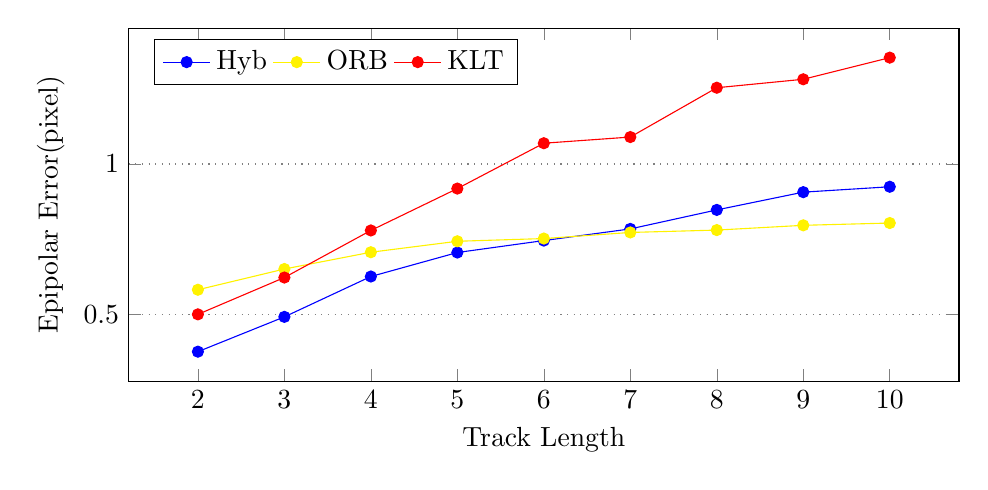
\begin{tikzpicture}
        \begin{axis}[
            xlabel={Track Length},
            ylabel={Epipolar Error(pixel)},
            legend pos=north west, % 图例位置
            legend columns=3, % 设置图例的列数为3
            grid=both, % 显示网格
            major grid style={dotted,gray}, % 主要网格线样式
            minor grid style={dotted,gray}, % 次要网格线样式
            xmajorgrids=false, % 不显示垂直主要网格线
            xminorgrids=false, % 不显示垂直次要网格线
            width=\linewidth, % 宽度设置为12厘米
            height=0.5\linewidth, % 高度设置为4厘米
            ]
            \addplot[color=blue,mark=*] coordinates {
                (2,0.374883)
                (3,0.490805)
                (4,0.625229)
                (5,0.705148)
                (6,0.744951)
                (7,0.783779)
                (8,0.84706)
                (9,0.906202)
                (10,0.924143)
                % (11,0.989535)
                % (12,0.973194)
                % (13,1.139)
                % (14,1.08904)
                % (15,1.14394)
                % (16,1.21185)
                % (17,1.10777)
                % (18,1.4823)
                % (19,1.19149)
                % (20,1.44675)
                % (21,1.43161)
                % (22,1.44882)
                % (23,1.50112)
                % (24,1.52332)
                % (25,1.5785)
            };
            \addlegendentry{Hyb}
            \addplot[color=yellow,mark=*] coordinates {
                (2,0.581117)
                (3,0.650189)
                (4,0.706101)
                (5,0.7426)
                (6,0.751624)
                (7,0.771983)
                (8,0.779857)
                (9,0.79575)
                (10,0.803329)
                % (11,0.808082)
                % (12,0.803262)
                % (13,0.79011)
                % (14,0.798317)
                % (15,0.779228)
                % (16,0.836509)
                % (17,1.0089)
                % (18,0.964484)
                % (19,0.840002)
                % (20,0.889293)
                % (21,0.769063)
                % (22,1.06872)
                % (23,0.855994)
                % (24,1.00139)
                % (25,1.0281)
            };
            \addlegendentry{ORB}
            \addplot[color=red,mark=*] coordinates {
                (2,0.499181)
                (3,0.62185)
                (4,0.778618)
                (5,0.918091)
                (6,1.06917)
                (7,1.08973)
                (8,1.25399)
                (9,1.28214)
                (10,1.35425)
                % (11,1.32911)
                % (12,1.45214)
                % (13,1.39665)
                % (14,1.56813)
                % (15,1.68793)
                % (16,1.74085)
                % (17,1.70084)
                % (18,1.73148)
                % (19,1.64343)
                % (20,1.60756)
                % (21,1.72251)
                % (22,1.91925)
                % (23,2.00618)
                % (24,2.09104)
                % (25,1.83422)
            };
            \addlegendentry{KLT}
        \end{axis}
    \end{tikzpicture}
    \caption{Epipolar error statistics on all data from EuRoC. The x-axis represents track length, and the y-axis indicates the median value of the epipolar error corresponding to the track length.}
    \label{fig:Epipolar_Error}
\end{figure}

% \begin{figure}
%     \centering
% \label{Track-Length}
%     \includegraphics[width=1\linewidth]{pictures/Track-Length.png}
%     \caption{Track length statistics for different sequences in EuRoC.}
%     \label{fig:track-length}
% \end{figure}

\begin{figure}[h]
    \centering
    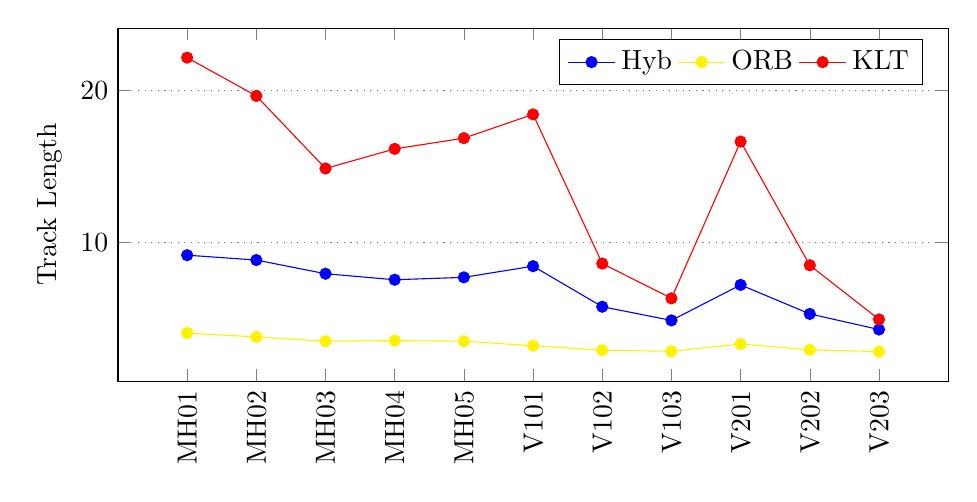
\begin{tikzpicture}
        \begin{axis}[
            % xlabel={Dataset},
            ylabel={Track Length},
            legend pos=north east, % 图例位置
            legend columns=3, % 设置图例的列数为3
            grid=both, % 显示网格
            major grid style={dotted,gray}, % 主要网格线样式
            minor grid style={dotted,gray}, % 次要网格线样式
            xmajorgrids=false, % 不显示垂直主要网格线
            xminorgrids=false, % 不显示垂直次要网格线
            width=\linewidth, % 宽度设置为12厘米
            height=0.5\linewidth, % 高度设置为4厘米
            xtick=data, % 使用数据点的值作为横坐标刻度
            xticklabels={MH01, MH02, MH03, MH04, MH05, V101, V102, V103, V201, V202, V203}, % 设置横坐标的标签
            xticklabel style={rotate=90,anchor=east,xshift=0cm}, % 标签旋转为垂直,锚点为东
            ]
            \addplot[color=blue,mark=*] coordinates {
                (1,9.16401)
                (2,8.84333)
                (3,7.94203)
                (4,7.54585)
                (5,7.70342)
                (6,8.44075)
                (7,5.76857)
                (8,4.86837)
                (9,7.20563)
                (10,5.2953)
                (11,4.26726)
            };
            \addlegendentry{Hyb}
            \addplot[color=yellow,mark=*] coordinates {
                (1,4.03109)
                (2,3.77664)
                (3,3.49368)
                (4,3.53465)
                (5,3.49801)
                (6,3.19997)
                (7,2.90238)
                (8,2.83099)
                (9,3.3095)
                (10,2.93061)
                (11,2.80861)
            };
            \addlegendentry{ORB}
            \addplot[color=red,mark=*] coordinates {
                (1,22.1775)
                (2,19.655)
                (3,14.8748)
                (4,16.1651)
                (5,16.8731)
                (6,18.4386)
                (7,8.61279)
                (8,6.32001)
                (9,16.6511)
                (10,8.50012)
                (11,4.93324)
            };
            \addlegendentry{KLT}
        \end{axis}
    \end{tikzpicture}
    \caption{Track length statistics for different sequences in EuRoC. Y-axis indicates the mean track length of each sequence.}
    \label{fig:track-length}
\end{figure}

To assess the effectiveness of the hybrid matching method, we conducted a comparative analysis using different matching strategies on the EuRoC dataset. These strategies include ORB's KNN matching, optical flow matching and hybrid matching. 

To evaluate the accuracy of feature matching, we employed the epipolar error metric. Using the true pose values provided by the dataset, we computed the relative pose between the two matched frames. Subsequently, with the relative pose and intrinsic parameters, we derived the fundamental matrix. The epipolar error metric is then calculated using the epipolar geometric relationship as follows:
\begin{equation}
        E_{epi} = \textbf{p}_i^T \textbf{F} \textbf{p}_j,
\end{equation}
where $\textbf{F}$ represents the fundamental matrix between frame $i$ and frame $j$ ,  and $\textbf{p}_i,\textbf{p}_j$ denote the corresponding feature points on the two frames.
We analyzed the relationship between track length and epipolar error across different feature matching methods using the entire EuRoC dataset. Specifically, \textit{ORB} denotes continuous frame KNN matching based on ORB features, \textit{KLT} signifies the optical flow method, and \textit{Hyb} represents our proposed hybrid method. From the results depicted in \cref{fig:Epipolar_Error}, it is observed that as the track length increases, the epipolar error also increases, indicating a positive correlation trend. Descriptor-based matching exhibits the smallest epipolar error, while optical flow-based matching demonstrates the largest epipolar error. Our hybrid matching method lies between them. Compared with optical flow matching, the hybrid method demonstrates a significant improvement in matching accuracy.

We further conducted statistical analysis on the track length of different matching strategies. In \cref{fig:track-length}, we observe that the optical flow-based method consistently yields longer track lengths across all sequences. However, these lengths exhibit significant fluctuations with changes in scene and movement speed. Additionally, as shown in \cref{fig:Epipolar_Error},  the long tracks produced by the KLT method may result in large epipolar errors, thereby not contributing to accuracy improvement. Our hybrid method maintains a moderate track length and exhibits stability across different sequences. Compared to the descriptor-based method, the track length of the hybrid approach shows a significant increase, nearly doubling.

We also compared the time consumption of the hybrid method and the KLT method in \cref{tab:time_statistics}. Despite the hybrid method utilizing both ORB and KLT in feature matching, the overall time consumption does not increase significantly. This is attributed to the shared feature detection module of ORB and KLT within the hybrid method, with the time-consuming increase primarily occurring in the matching process. Furthermore, leveraging the prior knowledge of KLT eliminates the need to extract an excessive number of ORB points (in our case, only 150 points are extracted), which proves adequate for matching within the sliding window. The time cost of \textit{others} includes triangulation, EKF filter, etc. 
\subsection{Trajectory Evaluation}
\begin{table*}[h]
    \caption{ATE (m)  of different algorithms on EuRoC.  Bold font indicates the best result in each column. '-' represents failure to run on this data. All results (except for HybVIO, whose ATE is obtained from \cite{hybvio}) were obtained by ourselves using open-source code and default configurations. None of them incorporate loop closure. }
    \centering
    \begin{tabular}{ccccccccccccc}
    \toprule
         & MH-01 & MH-02 & MH-03 & MH-04 & MH-05 & V1-01 & V1-02 & V1-03 & V2-01 & V2-02 & V2-03 & Avg. \\
         \midrule
         OKVIS      & 0.337 & 0.306 & 0.253 & 0.305 & 0.392 & 0.090 & 0.145 & 0.255 & 0.234 & 0.163 & 0.242 & 0.247 \\
         VINS-Mono  & 0.155 & 0.178 & 0.224 & 0.344 & 0.293 & 0.089 & 0.112 & 0.180 & 0.082 & 0.129 & 0.307 & 0.190 \\
         VINS-Fusion& 0.181 & 0.092 & 0.167 & 0.203 & 0.304 & 0.064 & 0.270 & 0.158 & 0.082 & -     & 0.160 & 0.168 \\
         OpenVINS   & \textbf{0.079} & 0.149 & 0.138 & 0.204 & 0.502 & 0.061 & 0.063 & \textbf{0.063} & 0.101 & \textbf{0.064} & 0.178 & 0.146 \\
         HybVIO     & 0.190 & \textbf{0.066} & \textbf{0.120} & 0.210 & 0.310 & 0.069 & 0.061 & 0.080 & \textbf{0.052} & 0.089 & 0.130 & 0.130 \\
         \midrule
         XR-VIO(KLT)& 0.106 & 0.144 & 0.145 & 0.230 & \textbf{0.212} & \textbf{0.050} & 0.044 & 0.100 & 0.073 & 0.071 & 0.158 & 0.121 \\
         XR-VIO(ORB)& 0.164 & 0.140 & 0.204 & 0.354 & 0.309 & 0.124 & 0.107 & 0.201 & 0.064 & 0.186 & 0.200 & 0.186 \\
         XR-VIO     & 0.082 & 0.114 & 0.164 & \textbf{0.181} & 0.215 & 0.060 & \textbf{0.041} & 0.075 & 0.062 & 0.081 & \textbf{0.100} & \textbf{0.107} \\
         \bottomrule
    \end{tabular}
    \label{tab:ATE_Compare}
\end{table*}
\begin{table*}[h]

    \caption{ATE (mm)  of different algorithms on the ZJU-Sensetime dataset. Bold font indicates the best result in each column. '-' represents failure to run on this data. XR-VIO (KLT) is the ablation version of our XR-VIO, utilizing only KLT for feature matching.}
    \centering
    \begin{tabular}{cccccccccc}
    \toprule
         &  A0&  A1&  A2&  A3&  A4&  A5&  A6&  A7& Avg.\\
         \midrule
         OKVIS\protect\footnotemark[1]          &  71.677 & 87.730 & 68.381 & 22.949 &  146.890 & 77.924 & 63.895 & 47.465 & 73.364 \\
         VINS-Mono\protect\footnotemark[1]      &  63.395 & 80.687 & 74.842 & 19.964 & 18.691 & 42.451 & 26.240 &  18.226 & 43.062 \\
         Vins-Fusion\protect\footnotemark[3]&  77.200 & 134.112 & 40.739 & 23.901 & 28.915 & 57.254 & 26.840 & 25.174 & 51.767\\
         OpenVINS\protect\footnotemark[3]& 74.368 & 97.339 & 41.610 & 22.387 & 16.862 & -   & 22.828 & 15.350 & 41.534\\
         HybVIO\protect\footnotemark[2]         &  \textbf{49.900}&  \textbf{30.000 }&  36.000&  22.200&  19.600&  37.800&  29.300&  17.300& 30.300\\
         SenseSLAM(V1.0)\protect\footnotemark[1]&  58.995 & 55.097 & 36.370 & 17.792 & 15.558 & 34.810 & 20.467 & \textbf{10.777} & 31.233\\
\hline
         XR-VIO(KLT)\protect\footnotemark[3]    &  \phantom{1}60.385\phantom{1} &  \phantom{1}71.926\phantom{1} &  \phantom{1}31.134\phantom{1} &  \phantom{1}16.657\phantom{1} &  \phantom{1}25.913\phantom{1} &  \phantom{1}34.288\phantom{1} &  \phantom{1}20.410\phantom{1} &  \phantom{1}13.125\phantom{1} & \phantom{1}34.230\phantom{1} \\
         XR-VIO(ORB)\protect\footnotemark[3]& 71.694 & 66.478 & 45.526 & 17.621 & 31.178 & 48.582 & 20.355 & 22.422 & 40.482\\
        XR-VIO\protect\footnotemark[3]          &  56.604 &  46.219 & \textbf{30.422} & \textbf{15.291}& \textbf{15.078}&  \textbf{30.283}& \textbf{17.082}&  12.598 & \textbf{27.947}\\
        \bottomrule
    \end{tabular}
    
    \label{tab:ATE_ZJU}
       \footnotemark[1]{ATE is obtained from \cite{jinyu2019survey}  }
       \footnotemark[2]{ATE is obtained from \cite{hybvio} }
       \footnotemark[3]{ATE is obtained by ourselves.}
\end{table*}

In \cref{tab:ATE_Compare,tab:ATE_ZJU}, we respectively compared our approach with the current state-of-the-art \cite{leutenegger-ijrr-2015-OKVIS, qin-tro-2018_VINS-Mono, qin2019a_VINS_Fusion_Local, geneva2020openvins,hybvio} on the EuRoC benchmark and the ZJU-Sensetime benchmark.
% \textit{All of these methods and our own run on same environment. Trajectories are without initialization part.}
% Our approach yields state-of-the-art performance on each dataset.
We also compared our own method with a baseline version employing solely KLT and ORB methods for feature matching, illustrating  the efficiency of our hybrid feature matching. The results demonstrate a noticeable improvement in ATE on both the EuRoC and ZJU-Sensetime datasets.

The ZJU-Sensetime dataset comprises data from consumer-grade mobile phones, captured with rolling cameras resulting in low-quality images often affected by motion blur. As a result, the accuracy of most algorithms is notably reduced when applied to this dataset. Our hybrid matching strategy demonstrates its advantage, particularly under the conditions present in the mobile phone dataset. Optical flow-based methods are particularly sensitive to variations in image quality, with rapid motion or changes in brightness causing significant errors in feature matching. However, our hybrid matching strategy effectively mitigates these issues, thereby improving the accuracy of VIO.
Additionally, more experimental results for accuracy comparison, such as evaluation on ADVIO \cite{cortes2018advio} dataset, can be found in our supplementary material.

In addition to the methods outlined in \cref{tab:ATE_Compare,tab:ATE_ZJU} , we refrain from comparing several other VIO/VI-SLAM systems, such as VI-ORB \cite{murartal-ral-2017-VI-ORB}, ORB-SLAM3 \cite{campos2021orb-slam3}, VI-DSO \cite{von2018direct-VI-DSO}, DM-VIO \cite{stumberg22DM-VIO}, despite their demonstrated high accuracy. This decision stems from their inherent latency issues, rendering them unsuitable for XR applications Latency manifests in two main aspects. Firstly, there is the computational burden. While algorithms in the ORB-SLAM series offer good accuracy, they rely on a significant number of complex calculations, making deployment on mobile platforms challenging. Secondly, there are delays inherent in the algorithm mechanisms. For instance, the ORB-SLAM\cite{murartal-ral-2017-VI-ORB, campos2021orb-slam3} series require 15 seconds of data to complete initialization, and DSO \cite{von2018direct-VI-DSO, stumberg22DM-VIO} series, with delayed marginalization, also need 2\textasciitilde10 seconds to obtain real scale. These latency issues are unacceptable for XR users.
\subsection{Ablation Study}
We conducted an ablation study on each initialization module under the 4KF configuration, as presented in \cref{tab:Ablation}. This analysis aimed to assess the individual impact of each module on initialization performance. The left column lists different algorithm strategies. \textit{Full} denotes our complete strategy for initialization, where all indicators demonstrate the best performance. Subsequently, we examined various ablation strategies. The ablation of \textit{2-point} demonstrates an improvement in the success rate of initialization. This method, when combined with known rotation, simplifies the solution for the initial relative pose. In contrast, the \textit{5-point} method requires solving complex polynomial problems and selecting the correct solution from a candidate set. \textit{VG-BA} represents an enhancement of traditional Visual-BA. By incorporating the orientation constraint of the gyroscope, the solution of the entire SfM problem becomes less prone to divergence, especially in cases of small motion and parallax. Moreover, VG-BA improves the accuracy of orientation estimation by optimizing gyroscope bias. Following VG-BA and initial visual-inertial alignment, the overall VI-BA plays a crucial role. The last two rows of \cref{tab:Ablation} demonstrate the impact of missing complete or partial VI-BA on initialization accuracy. Without VI-BA, scale error significantly increases, highlighting the importance of the weighting of visual terms.
\begin{table}[h]
    \centering

    \caption{Ablation study for VI-Initialization. Bold font indicates the best result, and Italic font highlights significant impact resulting from ablation.}
    \begin{tabular}{ccccc}
    \toprule
          &  Scale(\%)$\downarrow$&  ATE(m)$\downarrow$&  Gravity(°)$\downarrow$&  Succ(\%)$\uparrow$\\
          \midrule
           Full&  \textbf{26.88}&  \textbf{0.026}&  \textbf{2.26}&  \textbf{83.98}\\
           w/o 2-point&  27.08&  0.027&  2.34&  \textit{\textbf{80.43}}\\
           w/o VG-BA&  26.92&  0.027&  \textit{\textbf{2.45}} &  82.62\\
           w/o VI-BA&  \textit{\textbf{30.68}}&  0.028&  2.37&  83.98\\
          w/o weight&  \textit{\textbf{28.27}}&  0.028&  2.30&  83.84\\
    \bottomrule
    \end{tabular}
    \label{tab:Ablation}
\end{table}

\subsection{Mobile AR}
%We deployed our VIO system to mobile platforms (Android \& iOS) and developed a simple AR demo to demonstrate its accuracy and robustness. We utilized 30 Hz image data with a resolution of $640\times480$ and IMU data, including angular velocity and acceleration captured at 100/200Hz by the iPhone 13 Pro and Huawei Mate30 Pro. Our system operates in real-time on mobile devices, seamlessly integrating virtual objects into real-world scenes. \cref{fig:fancy AR demo} shows two AR examples. We assessed the accuracy of the algorithm by examining loop errors in the 3D trajectory during long-distance motion tracking in expansive scenes. Over tracking distances of several hundred meters, no visually significant loop errors or height discrepancies were observed. The experimental results demonstrate the superiority of our system in both initialization and normal tracking tasks, highlighting the effectiveness of our algorithm in XR applications. Further details of our mobile AR implementation can be found in our supplementary video material.
We deployed our VIO system on mobile platforms (Android \& iOS) and created a simple AR demo to showcase its accuracy and robustness. Using 30 Hz image data at a resolution of 640×480 and IMU data, including angular velocity and acceleration captured at 100/200Hz by the iPhone 13 Pro and Huawei Mate30 Pro, our system operates in real-time on mobile devices. It seamlessly integrates virtual objects into real-world scenes. \cref{fig:fancy AR demo} displays two AR examples. We evaluated the algorithm's accuracy by examining loop errors in the 3D trajectory during long-distance motion tracking in large scenes. Over distances of several hundred meters, no significant loop errors or height discrepancies were visually observed. The experimental results highlight the system's superior performance in both initialization and normal tracking tasks, emphasizing the algorithm's effectiveness in XR applications. Additional details of our mobile AR implementation are available in our supplementary video material.
\begin{figure}
    \centering
    \includegraphics[width=\columnwidth]{pictures/Mobile-AR.png}
    \caption{AR effects on mobile platforms}
    \label{fig:fancy AR demo}
\end{figure}
% \begin{figure}
%     \centering
%     \includegraphics[width=1\columnwidth]{pictures/Mobile-Trajectory.png}
%     \caption{Trajectory of VIO on a mobile phone: \textcolor{red}{need to add pic @nan, online AR + Trajectory}.}
%     \label{fig:fancy AR demo}
% \end{figure}

\section{Discussion}\label{sec:discussion}



\subsection{From Interactive Prompting to Interactive Multi-modal Prompting}
The rapid advancements of large pre-trained generative models including large language models and text-to-image generation models, have inspired many HCI researchers to develop interactive tools to support users in crafting appropriate prompts.
% Studies on this topic in last two years' HCI conferences are predominantly focused on helping users refine single-modality textual prompts.
Many previous studies are focused on helping users refine single-modality textual prompts.
However, for many real-world applications concerning data beyond text modality, such as multi-modal AI and embodied intelligence, information from other modalities is essential in constructing sophisticated multi-modal prompts that fully convey users' instruction.
This demand inspires some researchers to develop multimodal prompting interactions to facilitate generation tasks ranging from visual modality image generation~\cite{wang2024promptcharm, promptpaint} to textual modality story generation~\cite{chung2022tale}.
% Some previous studies contributed relevant findings on this topic. 
Specifically, for the image generation task, recent studies have contributed some relevant findings on multi-modal prompting.
For example, PromptCharm~\cite{wang2024promptcharm} discovers the importance of multimodal feedback in refining initial text-based prompting in diffusion models.
However, the multi-modal interactions in PromptCharm are mainly focused on the feedback empowered the inpainting function, instead of supporting initial multimodal sketch-prompt control. 

\begin{figure*}[t]
    \centering
    \includegraphics[width=0.9\textwidth]{src/img/novice_expert.pdf}
    \vspace{-2mm}
    \caption{The comparison between novice and expert participants in painting reveals that experts produce more accurate and fine-grained sketches, resulting in closer alignment with reference images in close-ended tasks. Conversely, in open-ended tasks, expert fine-grained strokes fail to generate precise results due to \tool's lack of control at the thin stroke level.}
    \Description{The comparison between novice and expert participants in painting reveals that experts produce more accurate and fine-grained sketches, resulting in closer alignment with reference images in close-ended tasks. Novice users create rougher sketches with less accuracy in shape. Conversely, in open-ended tasks, expert fine-grained strokes fail to generate precise results due to \tool's lack of control at the thin stroke level, while novice users' broader strokes yield results more aligned with their sketches.}
    \label{fig:novice_expert}
    % \vspace{-3mm}
\end{figure*}


% In particular, in the initial control input, users are unable to explicitly specify multi-modal generation intents.
In another example, PromptPaint~\cite{promptpaint} stresses the importance of paint-medium-like interactions and introduces Prompt stencil functions that allow users to perform fine-grained controls with localized image generation. 
However, insufficient spatial control (\eg, PromptPaint only allows for single-object prompt stencil at a time) and unstable models can still leave some users feeling the uncertainty of AI and a varying degree of ownership of the generated artwork~\cite{promptpaint}.
% As a result, the gap between intuitive multi-modal or paint-medium-like control and the current prompting interface still exists, which requires further research on multi-modal prompting interactions.
From this perspective, our work seeks to further enhance multi-object spatial-semantic prompting control by users' natural sketching.
However, there are still some challenges to be resolved, such as consistent multi-object generation in multiple rounds to increase stability and improved understanding of user sketches.   


% \new{
% From this perspective, our work is a step forward in this direction by allowing multi-object spatial-semantic prompting control by users' natural sketching, which considers the interplay between multiple sketch regions.
% % To further advance the multi-modal prompting experience, there are some aspects we identify to be important.
% % One of the important aspects is enhancing the consistency and stability of multiple rounds of generation to reduce the uncertainty and loss of control on users' part.
% % For this purpose, we need to develop techniques to incorporate consistent generation~\cite{tewel2024training} into multi-modal prompting framework.}
% % Another important aspect is improving generative models' understanding of the implicit user intents \new{implied by the paint-medium-like or sketch-based input (\eg, sketch of two people with their hands slightly overlapping indicates holding hand without needing explicit prompt).
% % This can facilitate more natural control and alleviate users' effort in tuning the textual prompt.
% % In addition, it can increase users' sense of ownership as the generated results can be more aligned with their sketching intents.
% }
% For example, when users draw sketches of two people with their hands slightly overlapping, current region-based models cannot automatically infer users' implicit intention that the two people are holding hands.
% Instead, they still require users to explicitly specify in the prompt such relationship.
% \tool addresses this through sketch-aware prompt recommendation to fill in the necessary semantic information, alleviating users' workload.
% However, some users want the generative AI in the future to be able to directly infer this natural implicit intentions from the sketches without additional prompting since prompt recommendation can still be unstable sometimes.


% \new{
% Besides visual generation, 
% }
% For example, one of the important aspect is referring~\cite{he2024multi}, linking specific text semantics with specific spatial object, which is partly what we do in our sketch-aware prompt recommendation.
% Analogously, in natural communication between humans, text or audio alone often cannot suffice in expressing the speakers' intentions, and speakers often need to refer to an existing spatial object or draw out an illustration of her ideas for better explanation.
% Philosophically, we HCI researchers are mostly concerned about the human-end experience in human-AI communications.
% However, studies on prompting is unique in that we should not just care about the human-end interaction, but also make sure that AI can really get what the human means and produce intention-aligned output.
% Such consideration can drastically impact the design of prompting interactions in human-AI collaboration applications.
% On this note, although studies on multi-modal interactions is a well-established topic in HCI community, it remains a challenging problem what kind of multi-modal information is really effective in helping humans convey their ideas to current and next generation large AI models.




\subsection{Novice Performance vs. Expert Performance}\label{sec:nVe}
In this section we discuss the performance difference between novice and expert regarding experience in painting and prompting.
First, regarding painting skills, some participants with experience (4/12) preferred to draw accurate and fine-grained shapes at the beginning. 
All novice users (5/12) draw rough and less accurate shapes, while some participants with basic painting skills (3/12) also favored sketching rough areas of objects, as exemplified in Figure~\ref{fig:novice_expert}.
The experienced participants using fine-grained strokes (4/12, none of whom were experienced in prompting) achieved higher IoU scores (0.557) in the close-ended task (0.535) when using \tool. 
This is because their sketches were closer in shape and location to the reference, making the single object decomposition result more accurate.
Also, experienced participants are better at arranging spatial location and size of objects than novice participants.
However, some experienced participants (3/12) have mentioned that the fine-grained stroke sometimes makes them frustrated.
As P1's comment for his result in open-ended task: "\emph{It seems it cannot understand thin strokes; even if the shape is accurate, it can only generate content roughly around the area, especially when there is overlapping.}" 
This suggests that while \tool\ provides rough control to produce reasonably fine results from less accurate sketches for novice users, it may disappoint experienced users seeking more precise control through finer strokes. 
As shown in the last column in Figure~\ref{fig:novice_expert}, the dragon hovering in the sky was wrongly turned into a standing large dragon by \tool.

Second, regarding prompting skills, 3 out of 12 participants had one or more years of experience in T2I prompting. These participants used more modifiers than others during both T2I and R2I tasks.
Their performance in the T2I (0.335) and R2I (0.469) tasks showed higher scores than the average T2I (0.314) and R2I (0.418), but there was no performance improvement with \tool\ between their results (0.508) and the overall average score (0.528). 
This indicates that \tool\ can assist novice users in prompting, enabling them to produce satisfactory images similar to those created by users with prompting expertise.



\subsection{Applicability of \tool}
The feedback from user study highlighted several potential applications for our system. 
Three participants (P2, P6, P8) mentioned its possible use in commercial advertising design, emphasizing the importance of controllability for such work. 
They noted that the system's flexibility allows designers to quickly experiment with different settings.
Some participants (N = 3) also mentioned its potential for digital asset creation, particularly for game asset design. 
P7, a game mod developer, found the system highly useful for mod development. 
He explained: "\emph{Mods often require a series of images with a consistent theme and specific spatial requirements. 
For example, in a sacrifice scene, how the objects are arranged is closely tied to the mod's background. It would be difficult for a developer without professional skills, but with this system, it is possible to quickly construct such images}."
A few participants expressed similar thoughts regarding its use in scene construction, such as in film production. 
An interesting suggestion came from participant P4, who proposed its application in crime scene description. 
She pointed out that witnesses are often not skilled artists, and typically describe crime scenes verbally while someone else illustrates their account. 
With this system, witnesses could more easily express what they saw themselves, potentially producing depictions closer to the real events. "\emph{Details like object locations and distances from buildings can be easily conveyed using the system}," she added.

% \subsection{Model Understanding of Users' Implicit Intents}
% In region-sketch-based control of generative models, a significant gap between interaction design and actual implementation is the model's failure in understanding users' naturally expressed intentions.
% For example, when users draw sketches of two people with their hands slightly overlapping, current region-based models cannot automatically infer users' implicit intention that the two people are holding hands.
% Instead, they still require users to explicitly specify in the prompt such relationship.
% \tool addresses this through sketch-aware prompt recommendation to fill in the necessary semantic information, alleviating users' workload.
% However, some users want the generative AI in the future to be able to directly infer this natural implicit intentions from the sketches without additional prompting since prompt recommendation can still be unstable sometimes.
% This problem reflects a more general dilemma, which ubiquitously exists in all forms of conditioned control for generative models such as canny or scribble control.
% This is because all the control models are trained on pairs of explicit control signal and target image, which is lacking further interpretation or customization of the user intentions behind the seemingly straightforward input.
% For another example, the generative models cannot understand what abstraction level the user has in mind for her personal scribbles.
% Such problems leave more challenges to be addressed by future human-AI co-creation research.
% One possible direction is fine-tuning the conditioned models on individual user's conditioned control data to provide more customized interpretation. 

% \subsection{Balance between recommendation and autonomy}
% AIGC tools are a typical example of 
\subsection{Progressive Sketching}
Currently \tool is mainly aimed at novice users who are only capable of creating very rough sketches by themselves.
However, more accomplished painters or even professional artists typically have a coarse-to-fine creative process. 
Such a process is most evident in painting styles like traditional oil painting or digital impasto painting, where artists first quickly lay down large color patches to outline the most primitive proportion and structure of visual elements.
After that, the artists will progressively add layers of finer color strokes to the canvas to gradually refine the painting to an exquisite piece of artwork.
One participant in our user study (P1) , as a professional painter, has mentioned a similar point "\emph{
I think it is useful for laying out the big picture, give some inspirations for the initial drawing stage}."
Therefore, rough sketch also plays a part in the professional artists' creation process, yet it is more challenging to integrate AI into this more complex coarse-to-fine procedure.
Particularly, artists would like to preserve some of their finer strokes in later progression, not just the shape of the initial sketch.
In addition, instead of requiring the tool to generate a finished piece of artwork, some artists may prefer a model that can generate another more accurate sketch based on the initial one, and leave the final coloring and refining to the artists themselves.
To accommodate these diverse progressive sketching requirements, a more advanced sketch-based AI-assisted creation tool should be developed that can seamlessly enable artist intervention at any stage of the sketch and maximally preserve their creative intents to the finest level. 

\subsection{Ethical Issues}
Intellectual property and unethical misuse are two potential ethical concerns of AI-assisted creative tools, particularly those targeting novice users.
In terms of intellectual property, \tool hands over to novice users more control, giving them a higher sense of ownership of the creation.
However, the question still remains: how much contribution from the user's part constitutes full authorship of the artwork?
As \tool still relies on backbone generative models which may be trained on uncopyrighted data largely responsible for turning the sketch into finished artwork, we should design some mechanisms to circumvent this risk.
For example, we can allow artists to upload backbone models trained on their own artworks to integrate with our sketch control.
Regarding unethical misuse, \tool makes fine-grained spatial control more accessible to novice users, who may maliciously generate inappropriate content such as more realistic deepfake with specific postures they want or other explicit content.
To address this issue, we plan to incorporate a more sophisticated filtering mechanism that can detect and screen unethical content with more complex spatial-semantic conditions. 
% In the future, we plan to enable artists to upload their own style model

% \subsection{From interactive prompting to interactive spatial prompting}


\subsection{Limitations and Future work}

    \textbf{User Study Design}. Our open-ended task assesses the usability of \tool's system features in general use cases. To further examine aspects such as creativity and controllability across different methods, the open-ended task could be improved by incorporating baselines to provide more insightful comparative analysis. 
    Besides, in close-ended tasks, while the fixing order of tool usage prevents prior knowledge leakage, it might introduce learning effects. In our study, we include practice sessions for the three systems before the formal task to mitigate these effects. In the future, utilizing parallel tests (\textit{e.g.} different content with the same difficulty) or adding a control group could further reduce the learning effects.

    \textbf{Failure Cases}. There are certain failure cases with \tool that can limit its usability. 
    Firstly, when there are three or more objects with similar semantics, objects may still be missing despite prompt recommendations. 
    Secondly, if an object's stroke is thin, \tool may incorrectly interpret it as a full area, as demonstrated in the expert results of the open-ended task in Figure~\ref{fig:novice_expert}. 
    Finally, sometimes inclusion relationships (\textit{e.g.} inside) between objects cannot be generated correctly, partially due to biases in the base model that lack training samples with such relationship. 

    \textbf{More support for single object adjustment}.
    Participants (N=4) suggested that additional control features should be introduced, beyond just adjusting size and location. They noted that when objects overlap, they cannot freely control which object appears on top or which should be covered, and overlapping areas are currently not allowed.
    They proposed adding features such as layer control and depth control within the single-object mask manipulation. Currently, the system assigns layers based on color order, but future versions should allow users to adjust the layer of each object freely, while considering weighted prompts for overlapping areas.

    \textbf{More customized generation ability}.
    Our current system is built around a single model $ColorfulXL-Lightning$, which limits its ability to fully support the diverse creative needs of users. Feedback from participants has indicated a strong desire for more flexibility in style and personalization, such as integrating fine-tuned models that cater to specific artistic styles or individual preferences. 
    This limitation restricts the ability to adapt to varied creative intents across different users and contexts.
    In future iterations, we plan to address this by embedding a model selection feature, allowing users to choose from a variety of pre-trained or custom fine-tuned models that better align with their stylistic preferences. 
    
    \textbf{Integrate other model functions}.
    Our current system is compatible with many existing tools, such as Promptist~\cite{hao2024optimizing} and Magic Prompt, allowing users to iteratively generate prompts for single objects. However, the integration of these functions is somewhat limited in scope, and users may benefit from a broader range of interactive options, especially for more complex generation tasks. Additionally, for multimodal large models, users can currently explore using affordable or open-source models like Qwen2-VL~\cite{qwen} and InternVL2-Llama3~\cite{llama}, which have demonstrated solid inference performance in our tests. While GPT-4o remains a leading choice, alternative models also offer competitive results.
    Moving forward, we aim to integrate more multimodal large models into the system, giving users the flexibility to choose the models that best fit their needs. 
    


\section{Conclusion}\label{sec:conclusion}
In this paper, we present \tool, an interactive system designed to help novice users create high-quality, fine-grained images that align with their intentions based on rough sketches. 
The system first refines the user's initial prompt into a complete and coherent one that matches the rough sketch, ensuring the generated results are both stable, coherent and high quality.
To further support users in achieving fine-grained alignment between the generated image and their creative intent without requiring professional skills, we introduce a decompose-and-recompose strategy. 
This allows users to select desired, refined object shapes for individual decomposed objects and then recombine them, providing flexible mask manipulation for precise spatial control.
The framework operates through a coarse-to-fine process, enabling iterative and fine-grained control that is not possible with traditional end-to-end generation methods. 
Our user study demonstrates that \tool offers novice users enhanced flexibility in control and fine-grained alignment between their intentions and the generated images.



%% if specified like this the section will be committed in review mode
% \acknowledgments{
% The authors wish to thank A, B, and C. This work was supported in part by
% a grant from XYZ.}

%\bibliographystyle{abbrv}
%\bibliographystyle{abbrv_conference/abbrv-doi}
\bibliographystyle{abbrv_journal/abbrv-doi}
%\bibliographystyle{abbrv-doi-narrow}
%\bibliographystyle{abbrv-doi-hyperref}
%\bibliographystyle{abbrv-doi-hyperref-narrow}

\bibliography{main}
\end{document}
